\documentclass{report}
\usepackage[spanish]{babel}
\usepackage[utf8]{inputenc}
\usepackage{graphicx, longtable, float, titlesec, hyperref, enumitem, dingbat, soul, multicol}
\usepackage[dvipsnames]{xcolor}
\usepackage[margin=3cm]{geometry}

% Cambia el color de los links
\hypersetup{
    hidelinks = true
}

% Elimina la palabra "Capítulo" de los títulos de los capítulos
\titleformat{\chapter}[display]
  {\normalfont\bfseries}{}{0pt}{\Huge\thechapter.\space}

\titleformat{name=\chapter,numberless}[display]
  {\normalfont\bfseries}{}{0pt}{\Huge}

\titlespacing*{\chapter}{0pt}{-50pt}{20pt}

% Añade numeración a los subsubsections y los añade al índice
\setcounter{secnumdepth}{4}
\setcounter{tocdepth}{4}

\begin{document}
    \begin{titlepage}
        \centering
        
\includegraphics[width=0.6\textwidth]{./img/logo.jpg}\\
        \vspace{1cm}
        \LARGE Sistemas de Apoyo a la Decisión\\
        \vspace{0.5cm}
        \Large Ingeniería Informática de Gestión y Sistemas de Información\\
        \vspace{3cm}
        \Huge Informe\\
        \huge LInUX\\
        \vspace{2.5cm}
        \Large Autores:\\
        \vspace{0.2cm}
        \large Xabier Gabiña\\
        \large Ibai Sologuestoa\\
        \large Unai Garcia\\
        \large Luken Bilbao\\
        \vfill
        \today
    \end{titlepage}
    \tableofcontents
    \listoffigures
    \listoftables
    \chapter*{Acrónimos}
        \begin{itemize}
            \item kNN: k-Nearest Neighbors
            \item LDA: Latent Dirichlet Allocation
        \end{itemize}
    \chapter{Tableau: Análisis de los Datos iniciales}
        \section{Introducción}
            \subsection{Bases}
                \paragraph*{}{
                Para comenzar el proyecto, a modo de base, se nos hace entrega de un conjunto de datos masivo, con información sobre opiniones de clientes de los último 7 años sobre aerolíneas cuyos servicios han utilizado. Estas opiniones incluyen información sobre el tipo de asiento del cliente que opina, su ruta de vuelo, la aerolínea, la clase en la que viajaba... así como sus opiniones sobre aspectos concretos del vuelo, como la comodidad del asiento o la calidad de la comida. 
                }
                \paragraph*{}{Estos datos, tras una serie de procesados y homologaciones, han sido convertidos en un conjunto coherente de datos que compara las opiniones de nuestra aerolínea (British Airlines} con nuestra principal competencia (Air France).
            \subsection{Objetivos}
                \paragraph*{}{El objetivo principal de este estudio es encontrar patrones y relaciones dentro de dichos datos para poder proporcionar a la dirección de nuestra empresa una estrategia de mejora en uno o varios aspectos de la compañía.}
        \section{Descripción de los datos}
            \begin{longtable}{|p{4cm}|p{4,7cm}|p{5,5cm}|}
                \hline
                \textbf{Titulo} & \textbf{Contenido}& \textbf{Descripcion}\\
                \hline
                Title & String, Cualitativo, Nominal & Breve descripcion de la review\\
                \hline
                Name & String, Cualitativo, Ordinal & Nombre del que ha hecho la review\\
                \hline
                Airline & String, Cualitativo, Nominal & Nombre de la aerolinina\\
                \hline
                Date & Date, Cualitativo, Nominal & Fecha de la review\\
                \hline
                Verified & Boolean, Cualitativo, Nominal & Verificado o no\\
                \hline
                Reviews & String, Cuantitativo, Discreto & Texto de la reseña\\
                \hline
                Type of Traveller & String, Cualitativo, Nominal & Tipo de viajero\\
                \hline
                Route & String, Cualitativo, Nominal & Recorrido del vuelo\\
                \hline
                Class & String, Cualitativo, Nominal & Tipo de clase del vuelo\\
                \hline
                Seat Confort & Int, Cuantitativo, Discreto & Comfort del asiento\\
                \hline
                Staff Service & Int, Cuantitativo, Discreto & Servicio del presonal\\
                \hline
                Food and Beverages & Int, Cuantitativo, Discreto & Comidas y bebidas\\
                \hline
                Inflight Entertainment & Int, Cuantitativo, Discreto & Entretenimiento\\
                \hline
                Value For Money & Int, Cuantitativo, Discreto & Valor por dinero\\
                \hline
                Overall Rating & String, Cuantitativo, Discreto & Calificacion general\\
                \hline
                Numerical Overall Rating & Int, Cuantitativo, Discreto & Puntuacion numérica\\
                \hline
                \caption{Descripción de los datos}
            \end{longtable}
            
        \section{Preprocesado de los datos}
            \paragraph*{}{A continuación, se describirán los distintos preprocesados a los que han sido sometidos los datos para su correcta representación en los gráficos de Tableau}
            \paragraph*{Formateado de fechas}{EL formato de las fechas de los datos de British Airlines (dd-mm-yyyy) para que se ajustara al formatos del resto de aerolíneas (M yyyy, siendo M el nombre del mes en inglés). En este proceso se perderá información, concretamente el día en el que se escribe la opinión, pero no usaremos esa información para la realización de ningún gráfico. El mes y el año serán suficientes.}
            \paragraph*{Eliminación o modificación de carácteres especiales}{En campos que contienen datos de tipo texto (como lo son los campos Title y Reviews), existe la presencia de carácteres que pueden dificultar el procesado de dicho texto. Por lo tanto, los carácteres de salto de línea, U+00a0, U+2013, "**" y carácteres en blanco al principio y al final de los campos se han eliminado o sustituido. Estos cambios no afectan al resultado de los gráficos ya que no utilizaremos este tipo de datos, pero es importante que todos los departamentos del equipo partamos de los mismos datos.}
            \paragraph*{Reestructuración de la ruta de vuelo}{Para poder hacer el map chart en Tableau, necesitaremos formatear la manera en la que se representan las rutas de vuelo de los aviones. Para esto inicialmente deberemos dividir la ruta en origen, destino y "vía", que reflejará en qué aeropuerto se hace escala. Además de esto y, aunque no se haya realizado este preproceso todavía, es probable que tengamos que homologar el nombre de los aeropuerto y transformarlos todos en sus respectivo código de tres letras (por ejemplo, Madrid sería MAD), para que Tableau pueda localizarlos en el mapa. Si esta cambio no es suficiente, puede que tengamos que introducir de alguna manera las coordenadas de dichos aeropuertos en el dataset.}
            \paragraph*{Opiniones negativas, neutras y positivas}{Aunque el dataset no nos de esta información, es preciso para conseguir unos gráficos comunicativos clasificar las opiniones de los usuarios en negativas, neutras y positivas, para poder centrarnos en las negativas, las cuales serán introducidas en este grupo por poseer una puntuación menor a 5.} 

        \section{Generación de gráficos}
            \subsection{¿Por qué un histograma?}
                \paragraph*{}{Un histograma es un tipo específico de gráfico que tiene como objetivo representar las características de distintos vectores de la muestra de datos. En nuestro caso, utilizaremos este tipo de gráficos para encontrar patrones de comportamiento en clientes pertenecientes a grupos concretos. Por ejemplo, podríamos ver a golpe de vista si muchos clientes que reservaron un asiento en primera clase han puesto una mala calificación en el apartado de "Comodidad de asiento". Estas conclusiones nos ayudarán a nosotros y a nuestra empresa a centrar nuestros esfuerzos en mejorar unos servicios concretos. En este caso, nuestra empresa se centraría en mejorar la comodidad de únicamente los asientos de primera clase, en vez de cambiar todos los asientos de todos los aviones, lo cual supondría un coste mucho mayor.}
            \subsection{¿Por qué un mapa?}
                \paragraph*{}{En nuestro caso particular, un mapa puede sernos de gran ayuda, al igual que los histogramas, a reconocer el origen de las malas reseñas y actuar con precisión consecuentemente. Nuestro map chart tendría como objetivo representar por medio de líneas las rutas que siguen los aviones de nuestra aerolínea, con el fin de dividir las opiniones de los usuarios según su ruta de vuelo. A través de esta representación, se nos brinda la oportunidad de ver representado en un mapa del globo que tan buenas o malas calificaciones reciben las distintas rutas que ofrece nuestra aerolínea. Esto nos permitirá, por ejemplo, identificar un patrón de malas reseñas hacia nuestro personal de cabina en una ruta entre dos ciudades concretas. De esta manera, podríamos tratar el problema con el staff que trabaje en esta ruta concreta directa y personalmente, en vez de dar una charla a todo el personal de cabina que posee la empresa, lo cual sería mucho más caro y, teniendo en cuenta lo poco directa e impersonal que sería dicha solución, probablemente menos efectiva.}
            \subsection{Selección de los gráficos} 
            \paragraph*{}{
            Dados los datos que tenemos, hemos generado un par de gráficos que creemos que son importantes destacar para incluir en los dashboards y en la historia. Para ver claramente la diferencia de rating entre British Airways y Air France, hemos generado un gráfico que representa las notas de las valoraciones entre las dos aerolíneas, siendo la línea roja Air France y la línea verde British Airways:
            }

            \begin{figure}[H]
                \centering
                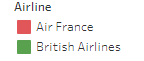
\includegraphics[width=0.3\textwidth]{img/Guion5.png}
                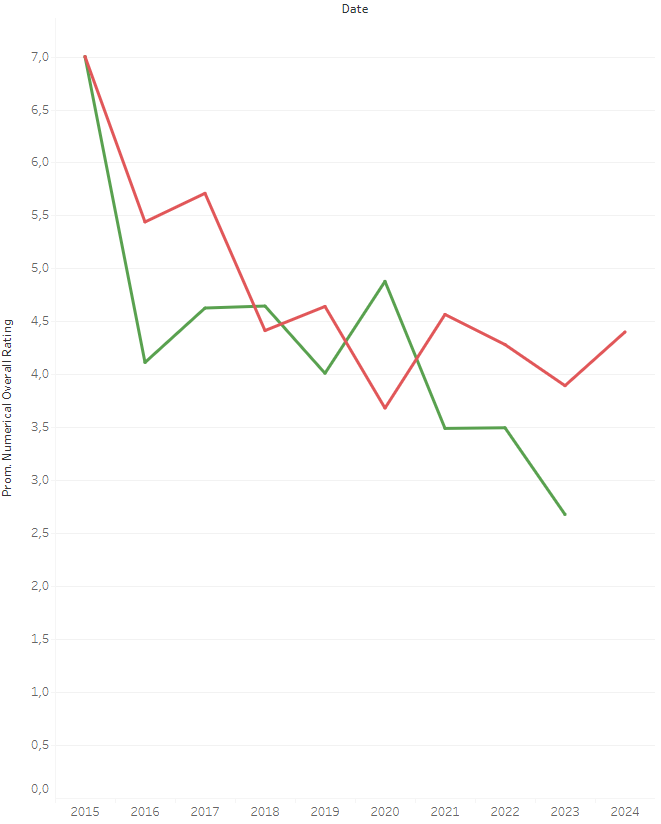
\includegraphics[width=0.5\textwidth]{img/Rating.png}
                \caption{Rating de British Airline y Air France}
            \end{figure}
                                                         
            \paragraph*{}{
            Aquí se pueden ver claramente que las dos compañías tuvieron unas críticas muy positivas en 2015, pero rápidamente bajaron; la bajada no fue tan grande para Air France como para British Airlines. Al contrario que la empresa francesa, nosotros mejoramos un poco, pero al año siguiente, al igual que nuestra competencia, las valoraciones bajaron de nota. En 2019, nuestras valoraciones incrementaron exponencialmente, mientras que las de Air France siguieron bajando, pero ya en 2020 los franceses empezaron a tener muy buenas valoraciones mientras que nosotros no. Las conclusiones que podemos tomar de esto es que en 2019 hicimos algo muy bueno que a la gente le gustó, pero en 2020 todo se fue al garete y no estamos sabiendo recuperarnos, mientras que Air France se está sabiendo adaptar.
            }
            \paragraph*{}{
            Algo que también hemos tenido en cuenta ha sido mirar si las valoraciones han sido verificadas o no, para evitar el sabotaje. Con este gráfico podemos verlo mejor, siendo el naranja las verificadas y el azul las que no:
            }
            \begin{figure}[H]
                \centering
                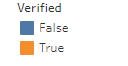
\includegraphics[width=0.3\textwidth]{img/Guion4.png}
                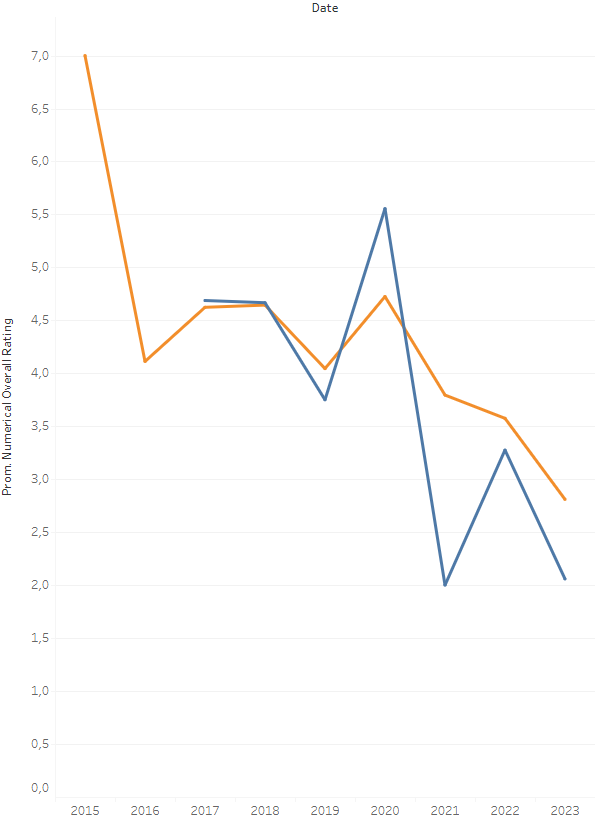
\includegraphics[width=0.5\textwidth]{img/Verified.png}
                \caption{Ratring de British Airline y Air France por estado de verificacion}
            \end{figure}
            

            
            \paragraph*{}{
            Viendo este gráfico, podemos observar que al principio, las valoraciones no verificadas nos mostraban opiniones positivas, pero ya en 2021 ha habido una oleada de reseñas negativas, lo que nos lleva a suponer que ha habido un sabotaje.
            }
            \paragraph*{}{
            Para ver más en resumen la cantidad de valoraciones negativas, medias y positivas, tenemos este gráfico resumen, siendo los rojos las críticas negativas, los naranjas las neutras y las verdes las positivas:
            }
            \begin{figure}[H]
                \centering
                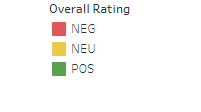
\includegraphics[width=0.3\textwidth]{img/Guion2.png}
                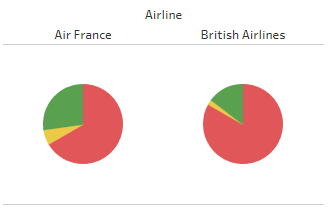
\includegraphics[width=0.5\textwidth]{img/Quesitos.png}
                \caption{Distribucion de valoraciones}
            \end{figure}
            
            \paragraph*{}{
            Aquí claramente podemos ver que tenemos peores críticas que nuestra competencia.
            }
            \paragraph*{}{
            Por último, tenemos un gráfico para ver las puntuaciones según las clases de vuelo:
            }
            \begin{figure}[H]
                \centering
                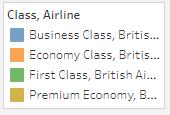
\includegraphics[width=0.3\textwidth]{img/Guion.png}
                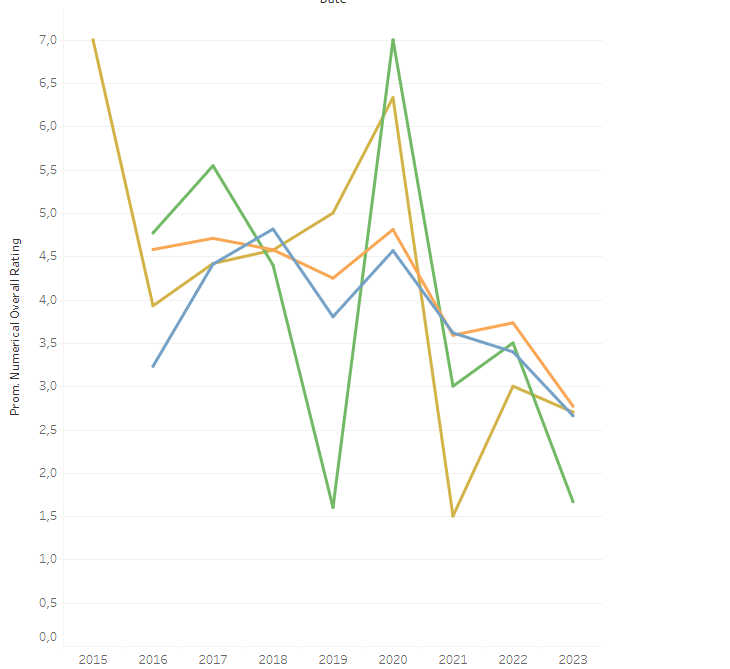
\includegraphics[width=0.5\textwidth]{img/Lineas.png}
                \caption{Valoraciones en base al tipo de vuelo}
            \end{figure}

            \paragraph*{}{
            Viendo esto, tenemos que mejorar sin duda la primera clase ya que las ultimas reviews esta siedo muy malas y por ultimo tendriamos que hacer cambios generales ya que todas las clases estan obteiendo malas criticas.
            }
    \chapter{Datos para clasificación: Análisis, Preproceso y Experimentación}
        \section{Datos}
            \subsection{División entre Train, Dev y Test}
                \paragraph*{Separación de Datos}{
                    Se ha separado los datos en Train y Dev en el programa con un split del 25\%. Esto asegura que tengamos suficientes datos para entrenar el modelo mientras reservamos una porción para la validación durante el desarrollo.
                }
                \paragraph*{Conjunto de Test}{
                    El conjunto de Test no se ha utilizado ya que no disponemos de el.
                }
            \subsection{Distribución de las clases en cada conjunto}
                \begin{longtable}{|c|c|c|}
                    \hline
                    \textbf{Conjunto De Datos} & \textbf{\% de instancias}& \textbf{Num. de instancias}  \\ \hline
                    Train & {75\%} & {6475}\\ 
                    \hline
                    Dev & {25\%} & {2158}\\ 
                    \hline
                    \caption{División Train y Dev}
                \end{longtable}
            \subsection{Distribución de las clases en cada conjunto}
                \begin{longtable}{|c|c|c|c|}
                \hline
                \textbf{Conjunto De Datos} & \textbf{Clase Neg} & \textbf{Clase Neutra}  & \textbf{Clase Pos.} \\ 
                \hline
                Train & {2891} & {601} & {2975}\\ 
                \hline
                Dev & {964} & {201} & {992}\\ 
                \hline
                \caption{Distribución Train y Dev}
                \end{longtable}
            \clearpage\subsection{Descripción del preproceso}
                \paragraph*{Droppear los datos} {
                     Al principio de la etapa de preprocesamiento, siguiendo los tres clasificadores planteados se eliminaron las columnas que no pertenecían a cada uno o simplemente sobraban. Se eliminaron aquellas características que no aportaban información relevante o que podían introducir ruido en los modelos predictivos como la fecha de las reseñas, los nombres de los usuarios que han escrito las reseñas y también hemos optado por droppear el tipo de avión, ya que solo aparece en el british.}
                \paragraph*{Separar los datos por tipos} {
                    Para facilitar el análisis y la aplicación de distintos métodos estadísticos y algoritmos de aprendizaje automático, se clasificaron las variables en tres categorías principales: numéricas, categóricas y de texto. Las variables \textbf{numéricas} incluyen aquellas que expresan cantidades y todo tipo de numero. Las variables \textbf{categóricas} representan grupos parecidos de texto que se van repitiendo y por último, las variables de \textbf{texto} contienen información en forma de cadenas de caracteres, las cuales requieren un procesamiento especial para su conversión y así ser utilizable en modelos predictivos. }
                \paragraph*{Simplificar el texto} {
                    Inicialmente, se verifica si hay columnas de texto para simplifica. Si es así, se procesara el texto de las respectivas columnas, primero se convierten todos los caracteres a minúsculas para estandarizar el texto, segundo se tokeniza el texto, es decir, se divide en palabras o tokens individuales, tercero se eliminan los números, cuarto se borran las palabras irrelevantes o stopwords en inglés, quinto se lematiza cada palabra para reducir las palabras a su raíz o forma base y finalmente, se eliminan los caracteres especiales como las diéresis que aparecen en palabras como Zürich que aunque en raras ocasiones aparecen. }
                \paragraph*{Convertir las columnas categóricas en numéricas} {
                    Se trabaja con las columnas que son categóricas, las que tienen un texto que se repite varias veces y que no tienen una gran cantidad de elementos diferentes, para ayudar a los modelos de aprendizaje lo que hacemos es coger las categorías de la columna y a cada valor diferente se le asigna un numero distinto y cada vez que en esa columna aparezca ese dato aparecerá ese numero, así hemos transformado correctamente una columna categórica a una numérica.}
                \paragraph*{Procesar los missing values} 
                { 
                    Cuando trabajamos con datos, es común encontrarnos con valores faltantes los cuales deben ser tratados para el correcto funcionamiento de nuestro modelo. 
                    Nuestras opciones son las siguientes:
                }
                \begin{itemize}
                    \item \textbf{Eliminar valores faltantes (Drop)}  
                    {En este metodo eliminamos las filas que contienen valores faltantes. Esto significa que si una fila tiene al menos un valor faltante en cualquiera de sus columnas, la eliminamos por completo.}
                    \item \textbf{Imputar con la media}  
                      {Reemplazamos los valores faltantes con la media de los valores existentes en esa columna.}
                    \item \textbf{Imputar con la mediana}  
                      {Este metodo es similar al anterior, pero usamos la mediana en lugar de la media.}
                    \item \textbf{Imputar con la moda}  
                      { Reemplazamos los valores faltantes con el valor más común en esa columna.}
                \end{itemize}
                \paragraph*{}{
                    Nosotros de todas las opciones implementadas hemos optado por usar el drop, ya que para las columnas de texto imputar puede resultar difícil, además es mas rápido y con la cantidad de filas existentes no debería ser un gran problema, aun así todas las opciones anteriores están implementadas aunque puede que den problemas con los textos.
                }
                \paragraph*{Reescalar los datos} {Los metodos de reescalados de datos que estan implementados son los siguientes:}
                \begin{itemize}
                    \item \textbf{MinMaxScaler}   
                        El método MinMaxScaler escala los datos llevándolos a un rango definido, generalmente entre 0 y 1. Esto se logra restando el valor mínimo de cada característica y luego dividiéndolo por el rango (valor máximo - valor mínimo). Es útil cuando los algoritmos requieren que los datos estén en un rango limitado o cuando no se puede operar con números negativos.
                    \item \textbf{Normalizer}   
                        El Normalizer, por otro lado, escala cada muestra, es decir, cada fila de la matriz de características, para tener una longitud unitaria. Esto se hace utilizando la norma euclidea, que es con la que funciona sklearn por defecto. Este tipo de escalado es útil cuando se quiere que las características contribuyan proporcionalmente al resultado final.
                    \item \textbf{MaxAbsScaler}   
                        MaxAbsScaler escala cada característica dividiendo cada valor por el valor absoluto máximo en esa característica. Esto tiene el efecto de situar los datos dentro del rango de -1 a 1
                    \item \textbf{StandardScaler}   
                        El StandardScaler, elimina la media y escala los datos a la varianza unitaria. Esto significa que convierte los datos en una distribución con una media de cero y una desviación estándar de uno.
                \end{itemize}
                \paragraph*{}{
                    Para realizar el análisis de sentimientos, hemos utilizado Naive Bayes, por lo tanto, el reescalado no es crucial, ya que este algoritmo no se ve tan afectado como lo estaría kNN. Sin embargo, hemos aplicado el escalador MinMax para mantener los datos en valores positivos, dado que el Multinomial Naive Bayes presenta problemas con datos negativos.
                }
                \paragraph*{Procesar el texto}{
                    El procesamiento de texto es un componente fundamental, ya que sin el, el texto no seria utilizable para entrenar nuestro modelo, nosotros tenemos implementados dos metodos de procesamiento de texto, los cuales son:
                }
                \paragraph*{TF-IDF}{
                      el cual es una técnica que refleja la importancia de una palabra en un documento en relación con una colección de documentos, el corpus. Funciona calculando la frecuencia de una palabra en un documento TF y multiplicándola por la inversa de la frecuencia de esa palabra en el corpus IDF. Esto ayuda a ajustar el valor de las palabras comunes que aparecen en muchos documentos y son menos informativas que las palabras que aparecen en menos documentos.
                }
                \paragraph*{BOW}{
                     es un modelo más simple que crea un saco de todas las palabras en los documentos, sin tener en cuenta el orden o la estructura del texto. Cada documento se representa como un vector en un espacio multidimensional donde cada dimensión corresponde a una palabra del corpus, y el valor en esa dimensión es la frecuencia de la palabra en el documento.
                }
                \paragraph*{}{
                    Nosotros por obvias razones hemos optado por utilizar el TF-IDF por ser un metodo más avanzado y el que nos puede dar mejores resultados a la hora de entrenar el modelo
                }    
            \clearpage\subsection{Primeros resultados}
                \paragraph*{}{
                Teniendo en cuenta que consideramos que después de hacer lo comentado en el apartado de muestreo se selecciona SMOTE para balancear las clases, ya que sin el como hemos visto en el apartado de distribución de las clases la clase neutra no estaria muy balanceada y podría resultar en menor capacidad de predicción de la anterior.
                }
                \paragraph*{}{
                Los primeros resultados que obtuvimos eran poco alentadores, probamos con diferentes algoritmos para probar sus respectivos rendimientos con nuestros datos, primero probamos a hacer kNN:
                }
                \begin{figure}[H]
                    \centering
                    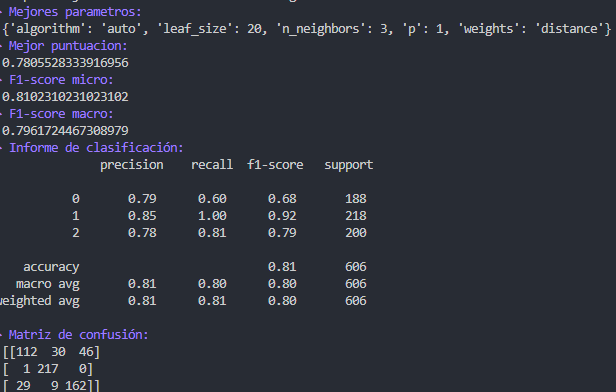
\includegraphics[width=0.7\textwidth]{img/kNNSMOTE.png}
                    \caption{Resultados de la ejecucion de kNN}
                \end{figure}
                \paragraph*{}{
                   Sorpresivamente los resultados son bastante positivos, aunque el tiempo de ejecución en este caso fue mucho mayor al de Naive Bayes, siguiendo nuestras pruebas decidimos ejecutar el algoritmo random forest el cual creemos que sera aun más positivo ya que se puede considerarse más complejo que el kNN:
                }
                \begin{figure}[H]
                    \centering
                    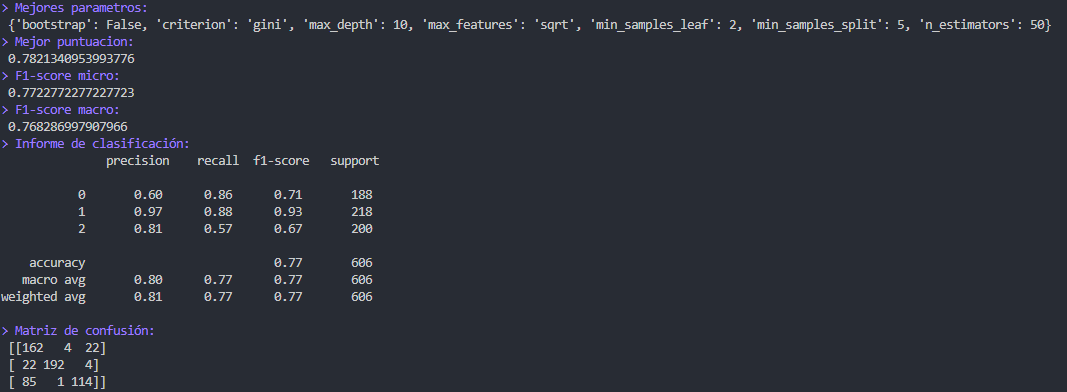
\includegraphics[width=0.7\textwidth]{img/randomForestSMOTE.png}
                    \caption{Resultados de la ejecucion de RandomForest}
                \end{figure}
                \paragraph*{}{
                Después de ejecutar el Random Forest observamos que la 'mejora' es casi inexistente, de hecho el F1 macro y micro se ven reducidos, por lo que ahora lo unico que nos toca es ejecutar el Naive Bayes:
                }
                \begin{figure}[H]
                    \centering
                    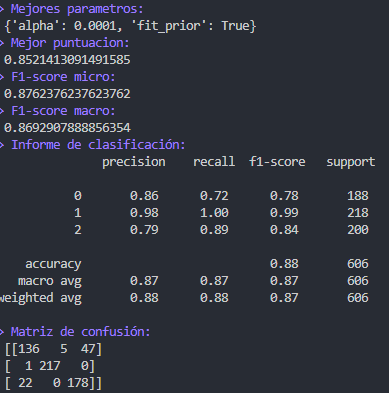
\includegraphics[width=0.7\textwidth]{img/SMOTE.png}
                    \caption{Resultados de la ejecucion de Naive Bayes}
                \end{figure}
                \paragraph*{}{
                    En donde si que vemos una mejora bastante en todos los apartados.
                }
               \paragraph*{}{
                   Hay que tener en cuenta que las 3 pruebas han sido ejecutadas con todos los datos, al hacerlo solo con el texto pierde puntuación y si es solo con los atributos aun más.
               }
            \clearpage\subsection{Descripción del Proceso de Submuestreo o Sobremuestreo}
                \paragraph*{}
                {
                    Al principio probamos con undersampling, porque creíamos que había suficientes datos como para poder reducir la cantidad y que el modelo aun pudiese seguir prediciendo correctamente, pero después de testear la teoría y obtener un resultado por debajo de lo esperado \color{red}{Peor puntacion:}
                }
                \begin{figure}[H]
                    \centering
                    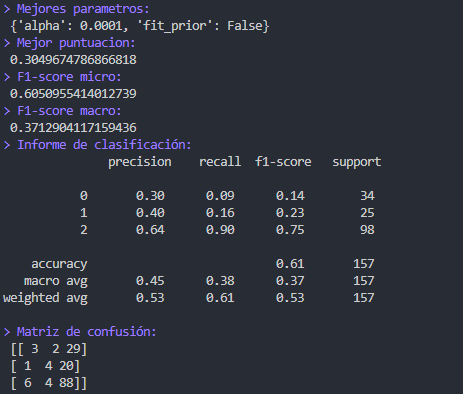
\includegraphics[width=\textwidth]{img/undersampling.png}
                    \caption{Resultados con undersampling}
                \end{figure}
                \paragraph*{}{
                    Decidimos optar por trabajar con oversampling, y aunque mejoro no era lo suficientemente bueno \color{orange}{Puntuacion media:}
                }
                \begin{figure}[H]
                    \centering
                    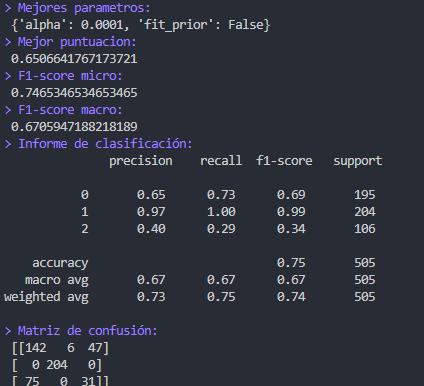
\includegraphics[width=\textwidth]{img/oversampling.png}
                    \caption{Resultados con oversampling}
                \end{figure}
                \paragraph*{}
                {
                    En ese momento nos vino a la cabeza el examen de laboratorio y decidimos usar la técnica SMOTE, la cual funciona como el oversampling pero en vez de ir repitiendo datos genera datos artificiales, lo que aumenta el ruido en nuestro en nuestro modelo y mejora contra el posible overfitting aunque todavía hay que tener cuidado, al usar el método comentado obtuvimos resultados muy positivos \color{green}{Mejor puntuacion:}
                }
                \begin{figure}[H]
                    \centering
                    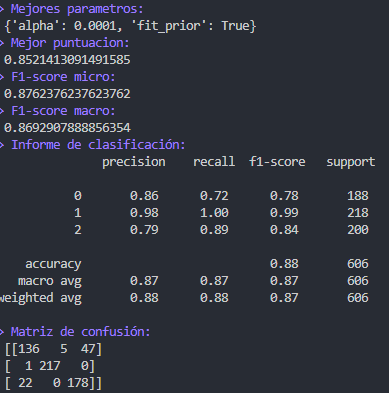
\includegraphics[width=\textwidth]{img/SMOTE.png}
                    \caption{Resultados con smote}
                \end{figure}
                \paragraph*{}{
                Siendo esta nuestra mejor opción, decidimos usar el metodo recien implementado para nuestro clasificador de sentimientos.
                }
        \clearpage\section{Algoritmos, link a la documentación y nombre de los hiperparámetros empleados}
            \subsection{Experimentación: Algoritmos empleados y Breve Descripción}
                \begin{itemize}
                    \item \textbf{Multinomial Naive Bayes}:
                    \begin{itemize}
                        \item Hiperparámetros: alpha: (0.00000001, 0.0001, 0.1, 0.25, 0.5, 0.75, 1.0, 2.0) y fit\_prior: (true, false)
                        \item Link: \href{https://scikit-learn.org/stable/modules/generated/sklearn.naive_bayes.MultinomialNB.html}{Sklearn MultinomialNB}
                    \end{itemize}
                \end{itemize}
                \paragraph*{}{
                Este modelo asume una distribución multinomial para la probabilidad de diferentes resultados y es efectivo para trabajar con características que representan frecuencias de eventos. En este caso el alpha es el smoothing de laplace y es lo que se suma para que los datos no tengan un 0 como probabilidad.
                }
                \begin{itemize}
                    \item \textbf{Random forest}:
                    \begin{itemize}
                         \item {Hiperparámetros: n\_estimators: (50), criterion: (gini), max\_depth: (5, 10), min\_samples\_split: (2, 5, 10), min\_samples\_leaf: (1, 2, 4), max\_features: (sqrt, log2), bootstrap: (false) }
                        \item Link: \href{https://scikit-learn.org/stable/modules/generated/sklearn.ensemble.RandomForestClassifier.html}{Sklearn Random Forest}
                    \end{itemize}
                \end{itemize}
                \paragraph*{} {
                Esta técnica opera mediante la creación de múltiples árboles de decisión para realizar predicciones más precisas. En esencia, cada árbol de decisión en el bosque considera una muestra aleatoria de los datos y realiza una votación sobre la predicción final, reduce mucho el posible overfitting causado por los decision trees. 
                }
                \begin{itemize}
                    \item\textbf{kNN}:
                    \begin{itemize}
                        \item {Hiperparámetros:n\_neighbors: (3, 5, 7, 9, 11), weights: (uniform, distance), algorithm: (auto), leaf\_size: (20, 30, 40), p: (1, 2)}
                        \item Link: \href{https://scikit-learn.org/stable/modules/generated/sklearn.neighbors.KNeighborsClassifier.html}{Sklearn kNN}
                    \end{itemize} 
                \end{itemize}
                \paragraph*{}{
                Este metodo se basa en clasificar un nuevo punto de datos basándose en la mayoría de votos de sus k vecinos más cercanos
                }
            \subsection{Conclusión sobre el Sentiment Analysis}
                \paragraph*{}{
                    Como conclusion decir que
                    hemos seleccionado el algoritmo Naive Bayes sobre Random Forest o KNN para el análisis de sentimientos de reseñas debido a varias razones clave. Primero, Naive Bayes es notablemente más rápido en términos de tiempo de entrenamiento y predicción, lo cual es crucial cuando se trabaja con grandes volúmenes de datos de texto. Además, a pesar de su simplicidad, Naive Bayes nos ha demostrado ser muy efectivo en tareas de clasificación de texto siendo el algoritmo que mejor resultados nos otorga. Por otro lado, modelos como Random Forest y KNN pueden ser computacionalmente costosos y menos eficientes en el manejo de datos de texto grandes.
                }
                \paragraph*{}{
                    La elección de SMOTE (Synthetic Minority Oversampling Technique) sobre métodos tradicionales de oversampling o undersampling en el análisis de sentimientos de reseñas se fundamenta en su capacidad para generar muestras sintéticas que ofrecen una representación más rica y diversa de la clase minoritaria. A diferencia del oversampling, que simplemente replica instancias existentes y puede conducir a un overfitting, SMOTE crea nuevas instancias sintéticas que ayudan a los modelos de aprendizaje automático a generalizar mejor. Por otro lado, el undersampling puede resultar en la pérdida de información valiosa al eliminar instancias de otras clases. SMOTE permite preservar esta información crítica mientras equilibra las clases, lo que resulta en un modelo más robusto y preciso para el análisis de sentimientos
                }
    \chapter{Datos para el Topic Modeling: Experimentación}
        \section{Algoritmos, link a la documentación y nombre de los hiperparámetros empleados}
            \begin{itemize}
                \item Algoritmos
                \begin{itemize}
                    \item Latent Dirichlet Allocation (LDA)
                    \item Non-Negative Matrix Factorization (NMF)
                \end{itemize}
                \item Link a la documentación
                \begin{itemize}
                    \item \href{https://radimrehurek.com/gensim/models/ldamodel.html}{Gensim - LDA Model}
                    \item \href{https://radimrehurek.com/gensim/auto_examples/tutorials/run_lda.html}{Gensim - Tutorial - Run LDA}
                    \item \href{https://radimrehurek.com/gensim/models/nmf.html}{Gensim - NMF Model}
                    \item \href{https://radimrehurek.com/gensim_3.8.3/models/nmf.html}{Gensim - Tutorial - NMF Model}
                    \item \href{https://radimrehurek.com/gensim/models/coherencemodel.html}{Gensim - Coherence Model}
                    \item \href{https://gensimr.news-r.org/articles/coherence}{Gensim - Article - Coherence}
                \end{itemize}
                \item Nombre de los hiperparámetros empleados
                \begin{itemize}
                    \item Title
                    \item Reviews
                \end{itemize}
            \end{itemize}
        \clearpage\section{Experimentación: Algoritmos empleados y breve descripción}
            \subsection{Preprocesado}
                \paragraph*{}{
                    Lo primero para realizar los experimentos de Topic Modeling es preprocesar los datos.
                    Dado que los algoritmos de Topic Modeling trabajan con texto, es necesario realizar un preprocesado muy enforcado en la limpieza de los mensajes.
                    Para ello, se han seguido los siguientes pasos:
                }
                \begin{enumerate}
                    \item Eliminar todas las columnas que no sean de texto.
                    \item Eliminarmos las filas que no contengan informacion.
                    \item Pasamos todo el texto a minúsculas
                    \item Tokenizamos el texto (dividimos el texto en palabras).
                    \item Borramos los números (ya que no aportan información en este caso)
                    \item Borramos las stopwords (palabras comunes que no aportan información).
                    \item Lemmatizamos el texto (reducimos las palabras a su raíz).
                    \item Unimos todas las columnas de texto en una sola (Gensim solo acepta un texto).
                    \item Generamos bigramas (se ha optado por no generar trigramas ya que no aportaban información en las pruebas realizadas).
                \end{enumerate}
                \paragraph*{}{
                    De esta forma obtenemos un texto limpio y listo para ser procesado por los algoritmos de Topic Modeling.
                }
                \paragraph*{}
                {
                    Para elegir el algoritmo a trabajar hemos tenido que elegir entre las dos categorías de algoritmos de clustering, \textit{``hard clustering"} y \textit{``soft clustering"}
                }
                \paragraph*{Los algoritmos Hard Clustering}{
                    suelen ser algoritmos mas sencillos y rápidos pero suelen ser menos precisos y \textbf{no permiten el solapamiento de topicos}, cualidad deseable para la tarea de Topic Modeling. A esta categoría pertenece el algoritmo \textbf{K-Means} y \textbf{Nearest Neighbors}.
                }
                \paragraph*{Los algoritmos Soft Clustering}{
                    son algoritmos más complejos y lentos pero permiten el solapamiento de topicos dado que la pertenencia de un documento es probabilistica y no binaria. A esta categoria pertenecen algoritmos como \textbf{LDA}, \textbf{NMF} o \textbf{GMM}.
                }
            \clearpage\subsection{Algoritmo de Asignación Latente de Dirichlet (LDA)}
                \paragraph*{}{
                    Con el texto preprocesado ya podemos aplicar el algoritmo elegido, LDA.
                    El algoritmo de Asignación Latente de Dirichlet (LDA, por sus siglas en inglés) es un método popular para el modelado de temas en un conjunto de documentos.
                    Su funcionamiento es el siguiente:
                }
                \begin{enumerate}
                    \item Se decide el número de temas que se quieren extraer.
                    \item Cada tema se representa como una distribución de palabras distribuida de forma aleatoria.
                    \item Cada documento se representa como una distribución de temas distribuida de forma aleatoria.
                    \item Para cada documento se recorre cada palabra y se calcula la probabilidad de que la palabra pertenezca a cada tema.
                    \item Se asigna a la palabra un nuevo tema basado en la probabilidad calculada.
                    \item Se repiten los pasos 3 y 4 hasta que converja.
                \end{enumerate}
                \paragraph*{}{
                    En este caso, la ejecucion del algoritmo corre a cargo de la librería Gensim, la cual nos proporciona una interfaz sencilla para trabajar con LDA.
                    Ademas, para evaluar la calidad de los temas generados, se ha utilizado la métrica de coherencia. 
                    La coherencia puede ser calculada de varias formas, nosotros, usaremos tanto \textbf{umass} como \textbf{c\_v}.
                    De esta forma podemos seleccionar el número de temas que mejor se ajuste a nuestros datos.
                }
                \paragraph*{}{
                    La ventaja de usar LDA es que es un \textbf{algoritmo no supervisado}, por lo que no necesita etiquetas para entrenar.
                    LDA es uno de los metodos más populares para el modelado de topicos debido a ser un \textbf{metodo probabilistico} y permitir el \textbf{solapamiento de topicos}. 
                    Además, es un algoritmo muy flexible y puede ser aplicado a cualquier conjunto de documentos.
                    Por otro lado, LDA tiene algunas desventajas. 
                    Por ejemplo, es un algoritmo muy lento y puede ser difícil de interpretar. 
                    Además, es difícil de ajustar y puede ser \textbf{difícil de converger}.
                }
            \subsection{Algoritmo de Factorización de Matrices No Negativas (NMF)}
                \paragraph*{}{
                    El algoritmo de Factorización de Matrices No Negativas (NMF, por sus siglas en inglés) es otro método popular para el modelado de temas en un conjunto de documentos.
                    Su funcionamiento es el siguiente:
                }
                \begin{enumerate}
                    \item Se decide el número de temas que se quieren extraer.
                    \item Se inicializan dos matrices, una que representa los documentos y otra que representa los temas.
                    \item Se calcula la distancia entre las dos matrices y se actualizan las matrices para minimizar la distancia.
                    \item Se repiten los pasos 2 y 3 hasta que converja.
                \end{enumerate}
                \paragraph*{}{
                    Al igual que con LDA, la ejecucion del algoritmo corre a cargo de Gensim.
                    Para evaluar la calidad de los temas generados, se ha utilizado la métrica de coherencia.
                    No obstante, los resultados obtenidos con NMF no han sido satisfactorios, por lo que hemos decidido centrarnos en LDA.
                }
        \clearpage\section{Resultados}
            \subsection{Resultados de British Airline}
                \subsubsection*{Valoraciones Positivas}
                    \paragraph*{}{
                        La primera muestra de datos sobre la que trabajaremos será la de las valoraciones positivas de nuestra empresa, British Airline.
                        Disponemos de un total de 403 valoraciones positivas, las cuales hemos procesado y analizado para extraer los temas más relevantes.
                        Para ello, hemos ejecutado nuestro algoritmo de LDA con distintos hiperparámetros \ref{tab:hiperparametros_british_airline_positivas} y hemos obtenido los siguientes resultados: 
                    }
                    \begin{figure}[H]
                        \centering
                        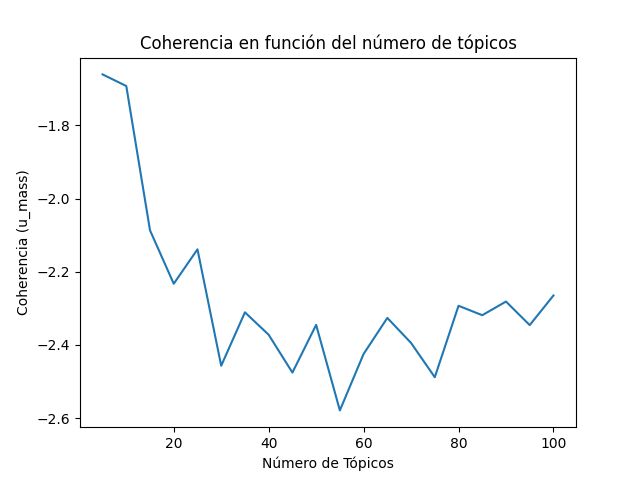
\includegraphics[width=0.49\textwidth]{./img/british_airline_positivas_umass.png}
                        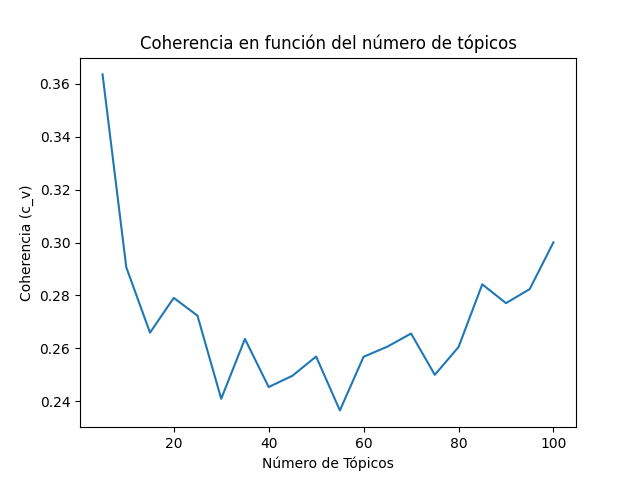
\includegraphics[width=0.49\textwidth]{./img/british_airline_positivas_cv.png}
                        \caption{Coherencia de las valoraciones positivas de British Airline}
                    \end{figure}
                    \paragraph*{}{
                        A pesar de que las graficas no son muy claras mostrando algun que otro diente de sierra, podemos intuir que el numero de temas optimos se encuentra entre el 20 y el 50.
                        En nuestro caso hemos ido con el valor de 30 ya que al analizar los temas obtenidos es el que hemos visto de forma más clara la interpretación de los mismos.
                    }
                \clearpage\subsubsection*{Valoraciones Neutra}
                    \paragraph*{}{
                        La segunda muestra de datos sobre la que trabajaremos será la de las valoraciones neutras de nuestra empresa, British Airline.
                        Disponemos de un total de 114 valoraciones neutras, las cuales hemos procesado y analizado para extraer los temas más relevantes.
                        Para ello, hemos ejecutado nuestro algoritmo de LDA con distintos hiperparámetros \ref{tab:hiperparametros_british_airline_neutras} y hemos obtenido los siguientes resultados:
                    }
                    \begin{figure}[H]
                        \centering
                        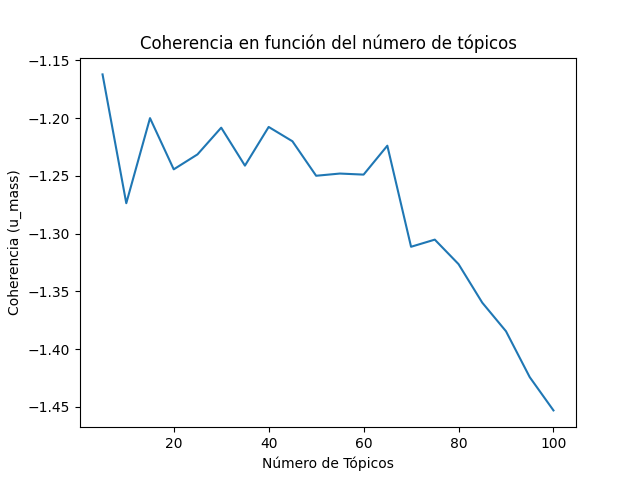
\includegraphics[width=0.49\textwidth]{./img/british_airline_neutras_umass.png}
                        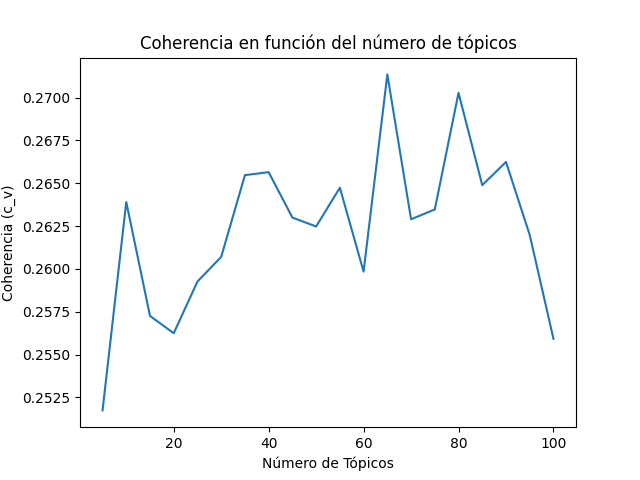
\includegraphics[width=0.49\textwidth]{./img/british_airline_neutras_cv.png}
                        \caption{Coherencia de las valoraciones neutras de British Airline primer intento}
                    \end{figure}
                    \paragraph*{}{
                        En este caso, las graficas son bastante diferentes entre si teniendo el c\_v bastantes picos en todo su recorrido.
                        La umass, en cambio, tiene un inicio bastante estable sobre todo a partir de los cinco topicos.
                        Esto y una lectura de los temas nos ha llevado a seleccionar el valor de 10 como el numero de topicos optimo.
                    }
                \clearpage\subsubsection*{Valoraciones Negativas}
                    \paragraph*{}{
                        La tercera muestra de datos sobre la que trabajaremos será la de las valoraciones negativas de nuestra empresa, British Airline.
                        Disponemos de un total de 810 valoraciones negativas, las cuales hemos procesado y analizado para extraer los temas más relevantes.
                        Para ello, hemos ejecutado nuestro algoritmo de LDA con distintos hiperparámetros \ref{tab:hiperparametros_british_airline_negativas} y hemos obtenido los siguientes resultados:
                    }
                    \begin{figure}[H]
                        \centering
                        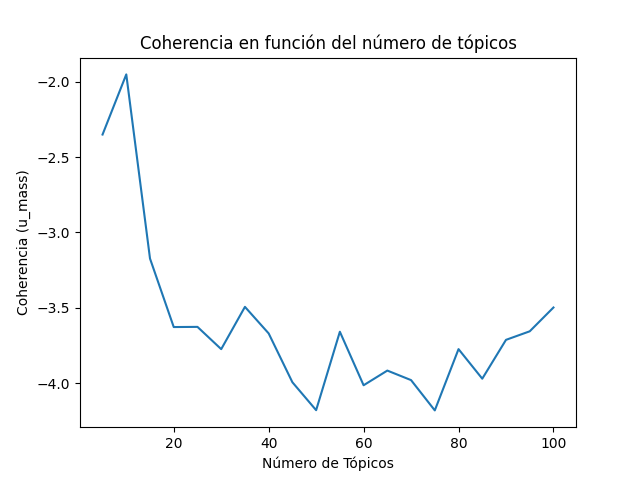
\includegraphics[width=0.49\textwidth]{./img/british_airline_negativas_umass.png}
                        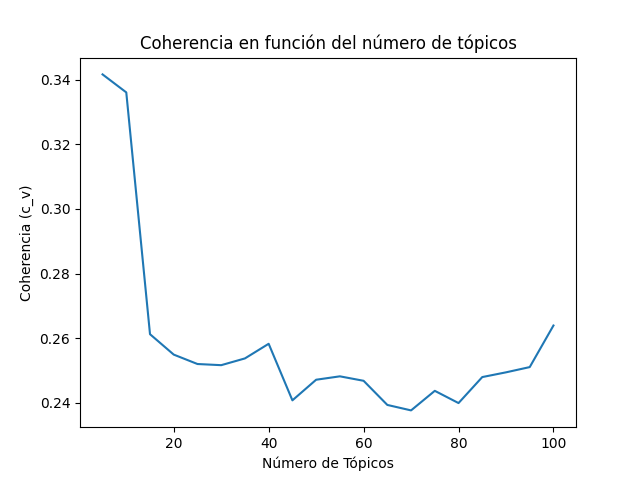
\includegraphics[width=0.49\textwidth]{./img/british_airline_negativas_cv.png}
                        \caption{Coherencia de las valoraciones negativas de British Airline}
                    \end{figure}
                    \paragraph*{}{
                        En esta ocasion ambas graficas son bastante parecidas y claras teniendo nada mas que dos posibles codos en nuestra opinion.
                        Uno inicial entre el 20 y el 40 y otro entre el 40 y el 60.
                        Al igual que en el resto de casos, hemos valorado la calidad de los temas obtenidos en los diferentes valores y hemos seleccionado el valor de 50 como el numero de topicos optimo.
                    }
            \clearpage\subsection{Resultados de Air France}
                \subsubsection*{Valoraciones Positivas}
                    \paragraph*{}{
                        La primera muestra de datos sobre la que trabajaremos será la de las valoraciones positivas de nuestra competencia, Air France.
                        Disponemos de un total de 305 valoraciones positivas, las cuales hemos procesado y analizado para extraer los temas más relevantes.
                        Para ello, hemos ejecutado nuestro algoritmo de LDA con distintos hiperparámetros \ref{tab:hiperparametros_air_france_positivas} y hemos obtenido los siguientes resultados:
                    }
                    \begin{figure}[H]
                        \centering
                        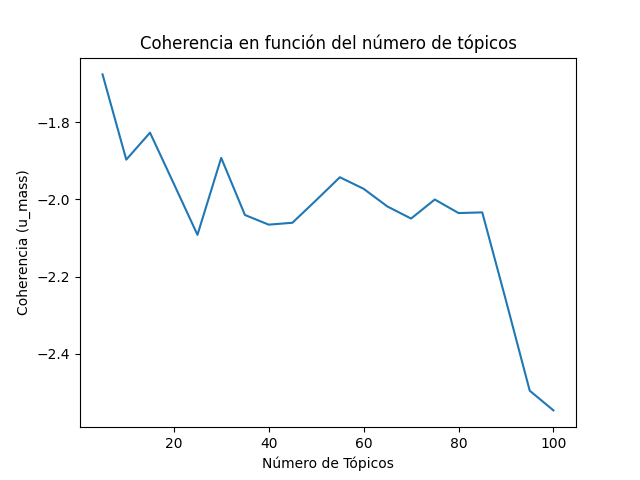
\includegraphics[width=0.49\textwidth]{./img/air_france_positivas_umass.png}
                        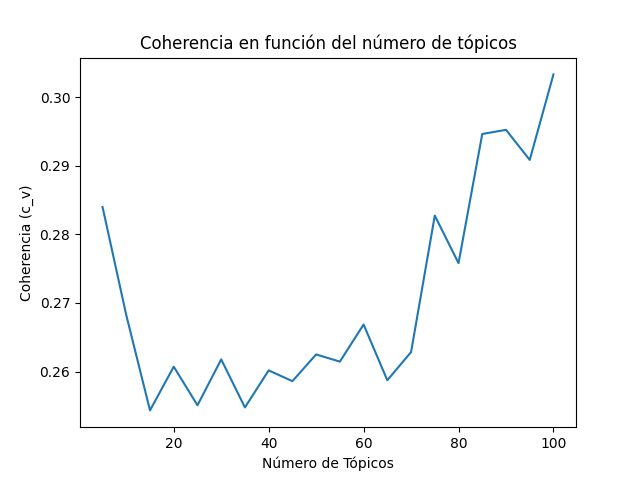
\includegraphics[width=0.49\textwidth]{./img/air_france_positivas_cv.png}
                        \caption{Coherencia de las valoraciones positivas de Air France primer intento}
                    \end{figure}
                    \paragraph*{}
                    {
                        En estas graficas podemos ver especialmente en la umass un codo bastante claro en el valor 40, punto, en el que en la grafica de c\_v marca un poco el limite antes de empezar a subir.
                        Es por esto que hemos seleccionado el valor de 40 como el numero de topicos optimo.
                    }
                \clearpage\subsubsection*{Valoraciones Neutra}
                    \paragraph*{}{
                        La segunda muestra de datos sobre la que trabajaremos será la de las valoraciones neutras de nuestra competencia, Air France.
                        Disponemos de un total de 53 valoraciones neutras, las cuales hemos procesado y analizado para extraer los temas más relevantes.
                        Para ello, hemos ejecutado nuestro algoritmo de LDA con distintos hiperparámetros \ref{tab:hiperparametros_air_france_neutras} y hemos obtenido los siguientes resultados:
                    }
                    \begin{figure}[H]
                        \centering
                        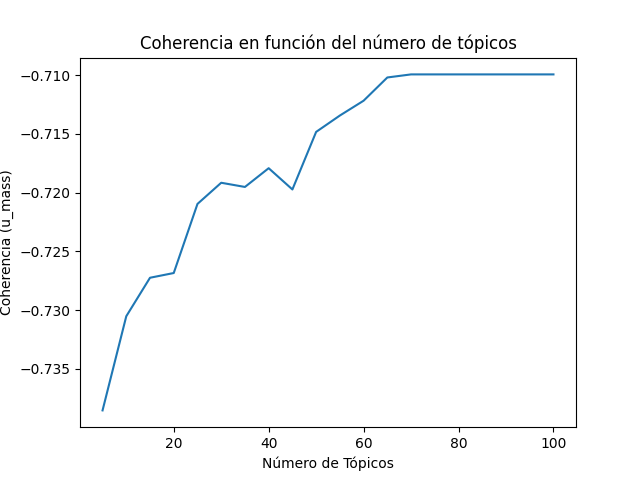
\includegraphics[width=0.49\textwidth]{./img/air_france_neutras_umass.png}
                        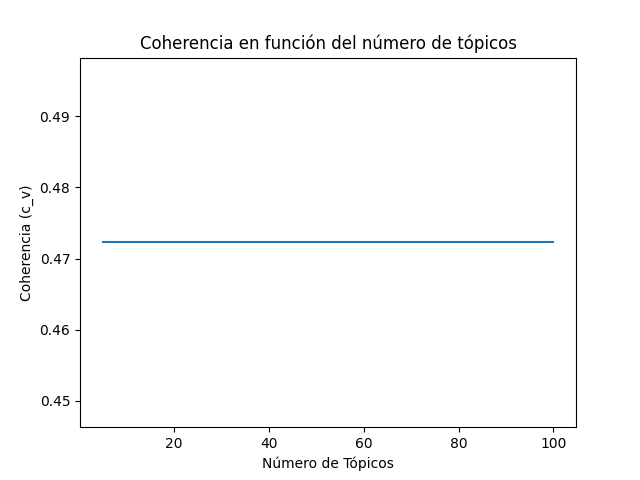
\includegraphics[width=0.49\textwidth]{./img/air_france_neutras_cv.png}
                        \caption{Coherencia de las valoraciones neutras de Air France primer intento}
                    \end{figure}
                    \paragraph*{}
                    {
                        En este caso poco vamos a poder sacar de los graficos debido al bajo numero de datos.
                        El umass no deja de subir y el c\_v tiene un valor constante en todo su recorrido.
                        Aunque hemos seleccionado el valor de 5 como el numero de topicos optimos, la realidad es que no se puede obtener nada de estos valores.
                    }
                \clearpage\subsubsection*{Valoraciones Negativas}
                    \paragraph*{}{
                        La tercera muestra de datos sobre la que trabajaremos será la de las valoraciones negativas de nuestra competencia, Air France.
                        Disponemos de un total de 443 valoraciones negativas, las cuales hemos procesado y analizado para extraer los temas más relevantes.
                        Para ello, hemos ejecutado nuestro algoritmo de LDA con distintos hiperparámetros \ref{tab:hiperparametros_air_france_negativas} y hemos obtenido los siguientes resultados:
                    }
                    \begin{figure}[H]
                        \centering
                        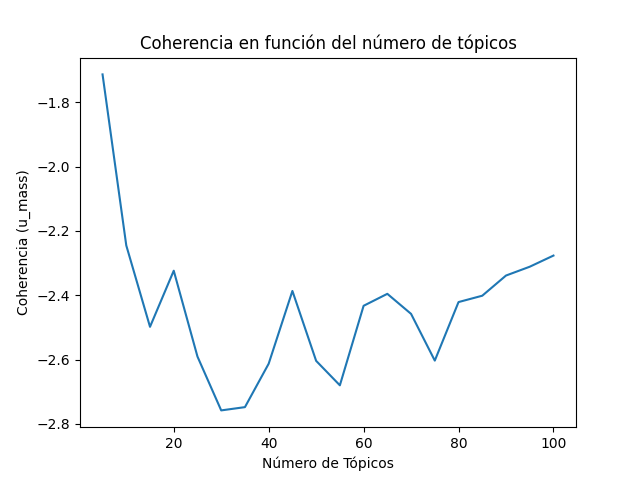
\includegraphics[width=0.49\textwidth]{./img/air_france_negativas_umass.png}
                        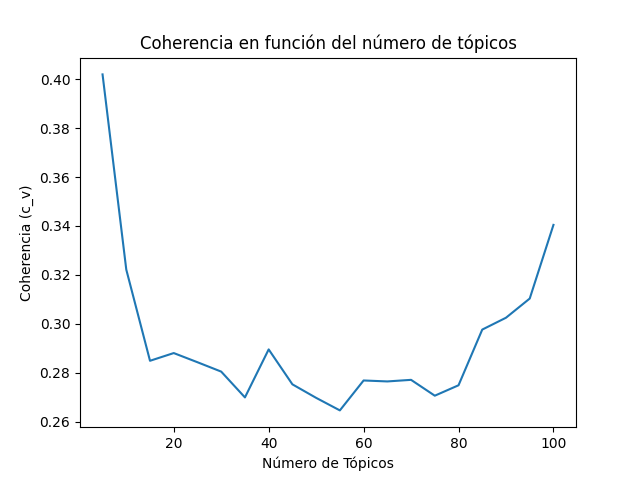
\includegraphics[width=0.49\textwidth]{./img/air_france_negativas_cv.png}
                        \caption{Coherencia de las valoraciones negativas de Air France}
                    \end{figure}
                    \paragraph*{}
                    {
                        En lo que respecta a estas graficas lo principal que puedo apreciar es que la grafica del c\_v se mantiene bastante estable en practicamente todo el recorrido especialmente entre los codos de los 20 y los 40 y los 60 y 80.
                        Tras analizar ambos codos hemos seleccionado el valor de 30 como el numero de topicos optimos principalmente porque los valores entre el 60 y 80 daban topicos repetidos o muy parecidos que apenas aportaban valor e incluso entorpecian la labor.
                    }            
        \clearpage\section{Discusión sobre los descubrimientos realizados en la tarea de Topic Modeling}
            \subsection{Descubrimientos sobre British Airline}
                \subsubsection*{Valoraciones positivas}
                    \paragraph*{}{
                        En general, la aerolínea ofrecen una experiencia premium con características que incluyen una tripulación amistosa, aviones cómodos y un sistema de entretenimiento robusto. Los vuelos de clase ejecutiva y primera clase destacan por sus menús de alta calidad y opciones de comidas y bebidas variadas, además de acceso a lounges exclusivos y abordaje temprano. Los vuelos de bajo costo brindan un servicio básico, pero pueden ofrecer un valor considerable para pasajeros con presupuestos ajustados.
                    }
                    \paragraph*{}{
                        El servicio a bordo suele ser amigable, aunque puede ser lento en ocasiones. Los problemas comunes incluyen retrasos, problemas con el equipaje y limitaciones de espacio, especialmente en clase económica. A pesar de esto, el personal de cabina a menudo se destaca por su amabilidad y disposición para ayudar. Los vuelos con el Airbus A380 tienden a ser más espaciosos y ofrecer mejores opciones de comida, aunque el servicio puede variar según la aerolínea.
                    }
                    \paragraph*{}{
                        El servicio en clase económica premium y económica estándar puede ser incómodo debido a la falta de espacio para las piernas, pero es apreciado por ser accesible y ofrecer entretenimiento a bordo. Los servicios en línea, como el check-in y el seguimiento de vuelos, facilitan el proceso, pero la comodidad y el horario de los vuelos pueden verse afectados por factores externos.
                    }
                    \paragraph*{}{
                        Todos los datos sobre los resultados de las valoraciones positivas de British Airline se encuentran en la tabla \ref{tab:temas_british_airline_positivas}.
                    }
                \subsubsection*{Valoraciones neutras}
                    \paragraph*{}{
                        Los vuelos en clase business y clase ejecutiva se destacan por su servicio personalizado y cabinas amplias, proporcionando un ambiente cómodo para los pasajeros. El acceso a lounges exclusivos y la oferta de comidas servidas contribuyen a una experiencia premium. Los pasajeros de clase ejecutiva tienden a valorar la calidad y eficiencia del servicio, notando la atención excepcional por parte del personal y la comodidad de las cabinas
                    }
                    \paragraph*{}{
                        Los vuelos desde y hacia el aeropuerto de Heathrow ofrecen una variedad de servicios que mejoran la experiencia del pasajero. Esto incluye un proceso de abordaje eficiente, inflight entertainment, y opciones de comida. El aeropuerto de Heathrow, en general, es conocido por tener un sistema de check-in eficiente y personal atento, lo cual agrega a la experiencia positiva del vuelo
                    }
                    \paragraph*{}{
                        En la clase económica, British Airways busca ofrecer un servicio de calidad que mantenga la comodidad del pasajero. Los vuelos de larga distancia ofrecen una variedad de opciones de entretenimiento y comidas, permitiendo a los pasajeros disfrutar de un viaje confortable. Los lounges y el servicio de cabina son vistos como lugares de comodidad, donde el personal es servicial y se ofrecen comodidades adicionales.
                    }
                    \paragraph*{}{
                        En la clase club, el servicio es eficiente y se brinda una experiencia premium, con comidas y bebidas que distinguen esta clase de la económica. Los pasajeros en esta clase suelen disfrutar de una tripulación dedicada, aviones modernos y servicios adicionales como inflight entertainment y cabinas más cómodas
                    }
                    \paragraph*{}{
                        En resumen, las valoraciones neutrales reflejan una experiencia generalmente positiva en vuelos de clase business y clase ejecutiva, especialmente en rutas desde y hacia el aeropuerto de Heathrow. El personal atento, el servicio eficiente y las comodidades ofrecidas, como inflight entertainment y opciones de comida, son aspectos valorados por los pasajeros
                    }
                    \paragraph*{}{
                        Todos los datos sobre los resultados de las valoraciones neutras de British Airline se encuentran en la tabla \ref{tab:temas_british_airline_neutras}.
                    }
                \subsubsection*{Valoraciones negativas}
                    \paragraph*{}{
                        El servicio y la actitud del personal son fuentes importantes de descontento. Si bien algunos pasajeros encuentran al personal amigable y servicial, muchas otras experiencias apuntan a actitudes negativas, falta de atención personalizada e inconsistencia en el servicio. Los pasajeros también informan dificultades con el proceso de check-in, así como con el embarque y desembarque
                    }
                    \paragraph*{}{
                        La calidad del equipamiento es otro punto de preocupación. Se menciona el uso de aviones desgastados y antiguos, lo que afecta tanto la comodidad como la experiencia de vuelo. Esto incluye quejas sobre asientos incómodos, espacio limitado y sistemas de entretenimiento que suelen ser anticuados y con opciones reducidas. En vuelos de clase económica y ejecutiva, las comodidades pueden ser escasas y el espacio para las piernas insuficiente, lo que genera incomodidad durante el viaje.
                    }
                    \paragraph*{}{
                        El manejo del equipaje y las largas esperas también contribuyen al descontento. Los pasajeros informan problemas con el equipaje perdido, así como retrasos y cancelaciones que afectan negativamente la experiencia general. Los vuelos de conexión y corta distancia suelen ser impredecibles, con demoras y problemas para coordinar el equipaje y el horario de los vuelos
                    }
                    \paragraph*{}{
                        En cuanto al inflight entertainment y otras comodidades a bordo, se destaca la falta de opciones y el mal funcionamiento de los sistemas, lo cual puede ser frustrante para los pasajeros. La falta de espacio, especialmente en vuelos de clase ejecutiva, y la calidad deficiente del servicio de catering son preocupaciones frecuentes
                    }
                    \paragraph*{}{
                        Los vuelos de aerolíneas de bajo costo tienden a ofrecer un servicio básico y limitado, sin atención personalizada. Los pasajeros también experimentan problemas con la coordinación del equipaje y el manejo de vuelos de conexión, lo que genera largas esperas y experiencias inconsistentes. Los vuelos de corta distancia con aerolíneas como EasyJet pueden ser particularmente incómodos debido a la estrechez de los asientos y la calidad del servicio
                    }
                    \paragraph*{}{
                        Finalmente, las experiencias durante las vacaciones pueden ser diversas, pero tienden a ser más negativas, con quejas sobre la falta de espacio y el mal servicio. Aunque algunos pasajeros encuentran aspectos positivos, como el esfuerzo por mantener un servicio razonable, las experiencias suelen ser variadas y a menudo decepcionantes.
                    }
                    \paragraph*{}{
                        En resumen, aunque se pueden encontrar experiencias positivas relacionadas con algunos servicios y personal, el panorama general sugiere una calidad inconsistente del servicio en British Airways, con problemas recurrentes que afectan significativamente la experiencia del pasajero.
                    }
                    \paragraph*{}{
                        Todos los datos sobre los resultados de las valoraciones negativas de British Airline se encuentran en la tabla \ref{tab:temas_british_airline_negativas}.
                    }
            \clearpage\subsection{Descubrimientos sobre Air France}
                \subsubsection*{Valoraciones positivas}
                    \paragraph*{}{
                        El servicio a bordo es a menudo destacado por su amabilidad y profesionalismo. Los pasajeros tienden a apreciar la atención del personal, quien proporciona una experiencia de cabina cómoda, alimentos de calidad y bebidas como vino y champán. Los vuelos en clase business, en particular, son elogiados por ofrecer cabinas amplias, comidas servidas y acceso a lounges exclusivos, lo que contribuye a un entorno premium y a una atención excepcional hacia el pasajero
                    }
                    \paragraph*{}{
                        El proceso de llegada y abordaje generalmente es eficiente y rápido, aunque algunos retrasos y problemas con el equipaje pueden surgir. Los vuelos desde y hacia el aeropuerto de Heathrow ofrecen un proceso de check-in eficiente y personal profesional, lo cual genera experiencias positivas para los pasajeros. En el caso de vuelos cortos y de clase económica, el servicio amigable y la comida suelen ser bien recibidos, aunque algunas experiencias mixtas pueden presentarse debido a la inconsistencia del servicio.
                    }
                    \paragraph*{}{
                        La calidad del inflight entertainment también es vista con buenos ojos, especialmente en vuelos de larga distancia, donde los pasajeros tienen acceso a una variedad de opciones. Aunque puede haber problemas con el equipaje y el proceso de embarque, el servicio a bordo suele ser profesional y amigable, con aviones limpios y comidas decentes. Los lounges también son mencionados por su eficiencia y comodidades, contribuyendo a una experiencia más agradable
                    }
                    \paragraph*{}{
                        Los vuelos desde Francia y París a menudo incluyen personal amable, servicios de comida agradables y un proceso de abordaje suave. Los vuelos de larga distancia pueden ser cómodos a pesar del espacio limitado, con opciones de comida y bebida que satisfacen a los pasajeros. Los aviones Boeing, en particular, son elogiados por su limpieza y personal profesional.
                    }
                    \paragraph*{}{
                        En resumen, las valoraciones positivas reflejan experiencias generalmente buenas en vuelos de clase business y clase económica. El servicio a bordo, la profesionalidad del personal y el proceso eficiente de check-in y abordaje son aspectos clave que contribuyen a una experiencia agradable para los pasajeros. A pesar de algunos problemas menores con el equipaje y el proceso de embarque, los pasajeros tienden a valorar el servicio amable y la calidad del inflight entertainment.
                    }
                    \paragraph*{}{
                        Todos los datos sobre los resultados de las valoraciones positivas de Air France se encuentran en la tabla \ref{tab:temas_air_france_positivas}.
                    }
                \subsubsection*{Valoraciones neutras}
                    \paragraph*{}{
                        El caso de las valoraciones neutras de Air France es un poco complicado dado a la pequeña muestra de las mismas.
                        Al no tener una cantidad suficiente de datos, no se puede realizar un análisis detallado de los temas encontrados dado que se repite el mismo topico continuamente.
                    }
                    \paragraph*{}{
                        De todas formas, esta valoracion parece ser positiva a pesar de que no se puede realizar un analisis detallado de los temas encontrados.
                    }
                    \paragraph*{}{
                        Todos los datos sobre los resultados de las valoraciones neutras de Air France se encuentran en la tabla \ref{tab:temas_air_france_neutras}.
                    }
                \subsubsection*{Valoraciones negativas}
                    \paragraph*{}{
                        Uno de los problemas más recurrentes se refiere al equipaje. Muchos pasajeros mencionan equipaje perdido, retrasos en la entrega de maletas, y problemas con el check-in y el manejo del equipaje. Estas dificultades no solo causan inconvenientes, sino que también afectan la experiencia general del viaje, generando frustración y malestar entre los pasajeros.
                    }
                    \paragraph*{}{
                        El servicio al cliente y el comportamiento del personal son otras áreas que preocupan a los pasajeros. Varios tópicos indican experiencias negativas con personal poco servicial y actitudes desagradables, tanto en los aeropuertos como a bordo de los aviones. Esto puede incluir desde falta de amabilidad hasta un trato grosero, lo que contribuye a una experiencia de viaje desfavorable.
                    }
                    \paragraph*{}{
                        Los retrasos y problemas con vuelos de conexión son una fuente de frustración adicional. Los pasajeros a menudo enfrentan vuelos retrasados, lo cual puede afectar la planificación de sus viajes y causar problemas para conexiones y otros arreglos. Estos retrasos también pueden generar estrés y ansiedad para los viajeros.
                    }
                    \paragraph*{}{
                        La calidad del servicio a bordo es otra preocupación destacada en los tópicos. Los pasajeros mencionan problemas con la calidad del inflight entertainment, comidas limitadas y aviones con equipos desgastados. Estos factores contribuyen a una experiencia de vuelo menos cómoda y satisfactoria, afectando la percepción general de la aerolínea.
                    }
                    \paragraph*{}{
                        Los problemas con la coordinación y el proceso de embarque son otros temas recurrentes. Los pasajeros pueden experimentar procesos de abordaje caóticos, largas esperas y falta de información clara sobre vuelos y conexiones. Estos problemas afectan la eficiencia del proceso de embarque y pueden resultar en experiencias negativas.
                    }
                    \paragraph*{}{
                        En cuanto al equipamiento de los aviones, se mencionan asientos incómodos, pantallas pequeñas y falta de espacio. Estos problemas afectan la comodidad y la experiencia a bordo, especialmente en vuelos de larga distancia. Además, las cancelaciones y demoras inesperadas agravan estas experiencias negativas, causando inconvenientes adicionales y afectando la satisfacción del pasajero.
                    }
                    \paragraph*{}{
                        En resumen, los tópicos indican que las experiencias negativas en vuelos y aerolíneas a menudo se centran en problemas con el equipaje, la calidad del servicio, los retrasos y el equipamiento deficiente. Estas preocupaciones recurrentes afectan significativamente la satisfacción del pasajero y su percepción general de la calidad del viaje.
                    }
                    \paragraph*{}{
                        Todos los datos sobre los resultados de las valoraciones negativas de Air France se encuentran en la tabla \ref{tab:temas_air_france_negativas}.
                    }
        \clearpage\section{Conclusión sobre la tarea de Topic Modeling}
            \paragraph*{}
            {
                La realidad es que British Airline tiene en su mayoria unas valoraciones negativas donde las principales quejas ordenadas por mas comunes son:
            }
            \begin{enumerate}
                \begin{multicols}{2}
                    \item Problemas con el servicio a bordo
                    \item Problemas con el equipamiento de los aviones
                    \item Problemas con el equipaje
                    \item Problemas con los servicios de entretenimiento
                    \item Problemas con el proceso de embarque
                    \item Problemas con los retrasos
                \end{multicols}
            \end{enumerate}
            Estos problemas son comunes en las aerolineas de bajo coste y suelen ser los principales motivos de queja de los pasajeros.
            No obstante, esto no quita que deban ser solucionados para mejorar la experiencia del pasajero y la percepción de la aerolinea en el mercado.
            \paragraph*{}
            {
                Air France, al igual que nosotros aunque en menor medida, tiene una cantidad de valoraciones negativas bastante elevada.
                Las principales quejas ordenadas por mas comunes son:
            }
            \begin{enumerate}
                \begin{multicols}{2}
                    \item Problemas con el equipaje
                    \item Problemas con el servicio a bordo
                    \item Problemas con los vuelos de conexión
                    \item Problemas con los servicios de entretenimiento
                    \item Problemas con el proceso de embarque
                    \item Problemas con el equipamiento de los aviones
                \end{multicols}
            \end{enumerate}
            \paragraph*{}
            {
                Como podemos ver, las quejas son las mismas para ambas compañias aunque en distinto orden.
                Esto es normal ya que ambas compañias operan en el mismo segmento de mercado y por lo tanto los problemas suelen ser comunes.
            }
            \paragraph*{}
            {
                Dado que ambas compañias flaquean en los mismos aspectos, considero que un factor diferencial para mejorar la percepción de la aerolinea en el mercado sería centrarse no solo en mejorar los puntos negativos si no potenciar los positivos.
                Por ejemplo, British Airline tiene una gran cantidad de valoraciones positivas sobre la clase ejecutiva y primera clase. 
                Tambien tiene una gran cantidad de valoraciones positivas sobre el servicio a bordo y sobre los costes de los vuelos.
                Potenciando estos aspectos y mejorando los negativos, British Airline podría mejorar su percepción en el mercado.
            }
            \paragraph*{}
            {
                Ademas podriamos adoptar algunas de las politicas de Air France que parece tener una mejor percepción en el mercado como podria ser los alimentos y bebidas servidos en los vuelos.
                Mejorar los procesos de embarque y abordaje y mejorar la calidad del servicio a bordo.
            }
            \paragraph*{}
            {
                Todos estos cambios deberian ser acompañados de una mejora en la comunicación con los pasajeros para que estos perciban que la aerolinea esta trabajando en mejorar y que sus opiniones son escuchadas.
                Lo que se traduciria en una mejora de la percepción de la aerolinea en el mercado y por lo tanto en un aumento de la cuota de mercado.
            }
    \chapter{Anexo}
        \section{Topic Modeling}
            \subsection{Hiperparámetros en las valoraciones positivas de British Airline}
                \label{tab:hiperparametros_british_airline_positivas}
                \begin{longtable}{|c|c|c|c|}
                    \hline
                    \textbf{Num Topics} & \textbf{Passes} & \textbf{Iterations} & \textbf{Coherence} \\
                    \hline
                    5 & 50 & 100 & -1.6609881786364327 \\
                    \hline
                    10 & 50 & 100 & -1.6926963155909387 \\
                    \hline
                    15 & 50 & 100 & -2.086815431759564 \\
                    \hline
                    20 & 50 & 100 & -2.23274273472322 \\
                    \hline
                    25 & 50 & 100 & -2.1386711042264706 \\
                    \hline
                    30 & 50 & 100 & -2.456646476860807 \\
                    \hline
                    35 & 50 & 100 & -2.3107740627829285 \\
                    \hline
                    40 & 50 & 100 & -2.3720305113919125 \\
                    \hline
                    45 & 50 & 100 & -2.47531929117352 \\
                    \hline
                    50 & 50 & 100 & -2.3450573553987737 \\
                    \hline
                    55 & 50 & 100 & -2.5786090745469608 \\
                    \hline
                    60 & 50 & 100 & -2.424467603766575 \\
                    \hline
                    65 & 50 & 100 & -2.325998201111187 \\
                    \hline
                    70 & 50 & 100 & -2.394396924546136 \\
                    \hline
                    75 & 50 & 100 & -2.488017140719314 \\
                    \hline
                    80 & 50 & 100 & -2.292882036431564 \\
                    \hline
                    85 & 50 & 100 & -2.318638285065557 \\
                    \hline
                    90 & 50 & 100 & -2.281340377764567 \\
                    \hline
                    95 & 50 & 100 & -2.3456530419909267 \\
                    \hline
                    100 & 50 & 100 & -2.2647457941363958 \\
                    \hline
                    \caption{Hiperparámetros en las valoraciones positivas de British Airline}
                \end{longtable}
            \clearpage\subsection{Temas encontrados en las valoraciones positivas de British Airline}
                \label{tab:temas_british_airline_positivas}
                \begin{longtable}{|p{1cm}|p{4cm}|p{4cm}|p{6cm}|}
                    \hline
                    \textbf{Id} & \textbf{Tema} & \textbf{Coherencia} & \textbf{Palabras} \\
                    \hline
                    1 & El servicio de British Airways destaca por su tripulación amistosa, aviones cómodos y atención a los pasajeros, brindando una experiencia premium. & -1.1039405713605002 & good, economy, crew, hour, staff, airway, british, plane, british\_airway, passenger, aircraft, one, experience, cabin, check, heathrow, time, friendly, premium, would \\
                    \hline
                    2 & Un vuelo bien equipado con un sistema de entretenimiento robusto, un personal profesional y una selección de alimentos y bebidas de alta calidad & -1.6432738924450339 & special, great, uncomfortable, water, system, working, point, new, experience, professional, excellent, entertainment, comfortable, lhr, well, dinner, good, clean, crew, wine \\
                    \hline
                    3 & La clase ejecutiva ofrece un gran menú, con opciones de desayuno y almuerzo, y asientos cómodos para vuelos largos & -1.6483561697078348 & club, really, meal, choice, leg, great, like, nice, served, cost, poor, way, flew, world, better, breakfast, last, water, trip, class \\
                    \hline
                    4 & La experiencia premium incluye acceso a lounges exclusivos, abordaje temprano y entretenimiento durante el vuelo para los pasajeros de clase alta & -1.880645233668626 & excellent, overall, lounge, ok, ground, world, good, arrival, entertainment, first, club\_world, premium, early, point, boarding, finally, u, arrived, fine, area \\
                    \hline
                    5 & El servicio de primera clase se distingue por su comodidad, aunque las opciones de entretenimiento y el sistema de clase pueden ser diferentes según la ruta. & -1.8929604598514909 & first\_class, looked, though, different, poor, system, last, first, day, low\_cost, route, low, flying, gatwick, carrier, class, cost, entertainment, year, offering \\
                    \hline
                    6 & Los pasajeros valoran la calidad del servicio a bordo, con un personal amable y una experiencia agradable durante todo el viaje. & -1.955177833402623 & getting, almost, everything, actually, nice, inflight, ticket, etc, make, go, special, really, quality, best, journey, good, board, know, behind, crew \\
                    \hline
                    7 & El servicio a bordo puede ser un poco lento, pero incluye opciones estándar de comida y bebida, con un ambiente relajado en la sala de espera. & -1.960193797927809 & slow, europe, schedule, food\_drink, standard, lounge, club, including, asked, arrival, usual, lunch, wine, although, minute, well, quick, old, hot, least \\
                    \hline
                    8 & Los problemas de vuelo, como retrasos en las rutas y problemas con el equipaje, pueden afectar el horario de los pasajeros. & -1.989271084280866 & gate, route, change, way, flown, day, luggage, issue, left, like, hour, time, little, journey, seating, check, see, much, early, toilet \\
                    \hline
                    9 & La tripulación es amigable y atenta, y se enfoca en brindar un servicio limpio y cómodo a los pasajeros durante el vuelo. & -2.130441406111533 & helpful, great, friendly, clean, fly, option, end, staff, aircraft, airline, best, attentive, enough, despite, decent, crew, feel, almost, lunch, need \\
                    \hline
                    10 & La experiencia en un vuelo con un Airbus A380 es agradable, aunque el itinerario y los horarios pueden ser ajustados para adaptarse al tráfico aéreo. & -2.141990799947005 & a380, nice, arrival, though, thing, schedule, lhr, window, inflight, full, trip, lounge, area, rest, served, like, ok, flying, terminal, film \\
                    \hline
                    11 & Los vuelos nocturnos pueden ser diferentes según la clase, con opciones para dormir, cenas y un servicio atento durante la noche. & -2.1640920691364847 & way, sleep, bag, different, come, without, dinner, night, via, flew, good, row, work, arrived, airways, class, travel, back, serving \\
                    \hline
                    12 & Los pasajeros aprecian la comodidad de la clase económica premium, con un servicio amigable y un sistema eficiente para abordar y desembarcar & -2.180466090197111 & nice, club, trip, helpful, economy, come, system, ground, best, also, class, comfortable, one, may, always, airport, serving, crew, last, old \\
                    \hline
                    13 & Los pasajeros tienen acceso a comida y bebida gratis, aunque las opciones pueden ser limitadas según la aerolínea y el tipo de vuelo & -2.2434115551992835 & go, food\_drink, free, glass, water, drink, little, though, luggage, looked, like, quality, give, u, good, etc, taking, low\_cost, fine, least \\
                    \hline
                    14 & El servicio en primera clase incluye opciones de desayuno y un ambiente exclusivo, aunque puede haber variaciones en el servicio según el itinerario & -2.2566670947771392 & little, longer, ground, first\_class, air, quite, attendant, economy, staff, breakfast, enough, serve, first, right, screen, different, could, checked, class, front \\
                    \hline
                    15 & Los pasajeros pueden enfrentar retrasos y tiempos de espera, pero el personal de cabina sigue siendo amable y servicial durante todo el proceso & -2.387216310850473 & delay, waiting, serve, got, passenger, hour, one, staff, never, despite, busy, easy, breakfast, cabin, early, said, ever, screen, full, security \\
                    \hline
                    16 & El espacio en clase económica puede ser estrecho y limitado, pero los pasajeros pueden optar por mejoras a clase premium para mayor comodidad & -2.4730989411969793 & point, especially, go, budget, extra, complaint, low\_cost, a380, sandwich, little, lunch, free, gatwick, luggage, haul, plus, within, short, need, leg \\
                    \hline
                    17 & El servicio de comidas incluye opciones de desayuno y cena, con un menú variado, aunque los precios pueden ser altos para algunos servicios adicionales & -2.484532317167532 & breakfast, served, bar, cheese, landing, paid, anything, last, second, available, board, around, part, extra, ticket, want, short, get, price, menu \\
                    \hline
                    18 & Los vuelos de bajo costo ofrecen un servicio básico, con opciones de presupuesto y extras pagados, pero pueden faltar ciertos servicios premium & -2.513078464344632 & low\_cost, product, standard, little, extra, low, budget, like, card, pay, expect, including, airline, clean, bit, boarding, even, everything, outbound, paying \\
                    \hline
                    19 & El servicio de clase ejecutiva brinda comodidad y atención al detalle, con un personal atento y un servicio eficiente durante el vuelo & -2.5299178009334486 & via\_london, charge, late, arrived, know, via, even, air, business\_class, due, ife, friendly, business, helpful, attendant, middle, attentive, window, class, schedule \\
                    \hline
                    20 & Los pasajeros pueden encontrar algunas áreas incómodas en el avión, pero el personal de cabina trabaja para mantener la limpieza y la seguridad & -2.6111642993348205 & via\_london, ground, complaint, clean, via, second, different, water, taking, actually, paying, without, menu, uncomfortable, plane, old, cabin\_crew, bit, cabin, passenger \\
                    \hline
                    21 & El costo y la comodidad del servicio en clase económica premium pueden ser problemas, pero los clientes valoran la atención y las comodidades adicionales a bordo & -2.64990665089828 & issue, price, nothing, especially, complaint, review, onboard, comfort, enough, quite, customer, extra, premium\_economy, much, really, plus, special, economy, premium, poor \\
                    \hline
                    22 & Los pasajeros experimentan una mezcla de servicios en vuelos cortos, desde inflight entertainment hasta asientos cómodos, con algunos aspectos mejorables & -2.73599956999537 & quite, inflight, helpful, nothing, review, best, average, everything, short, comfortable, felt, flew, bad, cost, bed, breakfast, provided, thing, left, lot \\
                    \hline
                    23 & El espacio en clase business en aviones Boeing puede ser estrecho y ofrecer una experiencia menos confortable, lo que genera críticas negativas & -2.9375962813935304 & far, especially, boeing, review, bad, small, seating, business\_class, part, cramped, club, class, never, worst, may, ok, attendant, feel, one, new \\
                    \hline
                    24 & Los vuelos de bajo costo ofrecen un servicio básico, con opciones limitadas de comida y espacio, pero algunas aerolíneas brindan un servicio decente a un precio más bajo & -2.98306397113935 & low\_cost, serve, go, taking, despite, though, carrier, especially, inflight, a380, sandwich, narrow, part, row, outbound, call, every, flew, space, option \\
                    \hline
                    25 & La clase económica puede ser incómoda debido a la falta de espacio para las piernas, pero los pasajeros aprecian el precio accesible y el entretenimiento a bordo & -2.984323251621676 & budget, different, rest, comfortable, pleasant, enough, really, legroom, charge, leg\_room, would, film, plus, trip, issue, window, small, fly, part, top \\
                    \hline
                    26 & Los vuelos de bajo costo pueden ser una opción económica, pero a veces se deben tomar decisiones basadas en el presupuesto y la comodidad adicional & -3.0433688948204325 & point, especially, go, budget, extra, complaint, low\_cost, a380, sandwich, little, lunch, free, gatwick, luggage, haul, plus, within, short, need, leg \\
                    \hline
                    27 & Los servicios en línea, como el check-in y el seguimiento de vuelos, facilitan el proceso de vuelo, pero el tiempo de vuelo puede variar según la ruta & -3.072550090816227 & online, carrier, charge, short, low, schedule, choice, check, inflight, way, london\_heathrow, may, rather, small, quite, onboard, offering, okay, outbound, part \\
                    \hline
                    28 & Los pasajeros valoran la rapidez del servicio y el trato amistoso, pero el espacio limitado en algunos aviones puede ser un inconveniente para ciertos vuelos & -3.412211470918494 & luggage, quick, narrow, t5, free, water, old, right, time, finally, point, friendly, holiday, complaint, menu, top, actually, outbound, decided, staff \\
                    \hline
                    29 & La experiencia en vuelos con el Airbus A380 ofrece ventajas como mayor espacio y mejores opciones de comida, pero algunos aspectos, como el servicio, pueden variar según la aerolínea & -3.431906811191779 & a380, sandwich, plus, lunch, fine, change, journey, finally, though, home, enough, schedule, little, club\_world, world, always, club, luggage, quite, europe \\
                    \hline
                    30 & Los pasajeros encuentran aspectos positivos como el manejo del equipaje y la flexibilidad en el servicio, pero puede haber problemas de horarios y cambios inesperados en algunos vuelos & -4.258571121187838 & luggage, little, though, fine, enough, inflight, journey, second, home, least, always, schedule, actually, especially, complaint, looked, part, taking, change, something \\
                    \hline
                    \caption{Temas encontrados en las valoraciones positivas de British Airline}
                \end{longtable}
            \clearpage\subsection{Hiperparámetros en las valoraciones neutras de British Airline}
                \label{tab:hiperparametros_british_airline_neutras}
                \begin{longtable}{|c|c|c|c|}
                    \hline
                    \textbf{Num Topics} & \textbf{Passes} & \textbf{Iterations} & \textbf{Coherence} \\
                    \hline
                    5 & 50 & 100 & -1.1620576197099193 \\
                    \hline
                    10 & 50 & 100 & -1.2736384499672275 \\
                    \hline
                    15 & 50 & 100 & -1.1999287235764515 \\
                    \hline
                    20 & 50 & 100 & -1.2442886957358574 \\
                    \hline
                    25 & 50 & 100 & -1.231358395506873 \\
                    \hline
                    30 & 50 & 100 & -1.2081969944171325 \\
                    \hline
                    35 & 50 & 100 & -1.2410798263372813 \\
                    \hline
                    40 & 50 & 100 & -1.2075726814313836 \\
                    \hline
                    45 & 50 & 100 & -1.2199556524612487 \\
                    \hline
                    50 & 50 & 100 & -1.2498548816351787 \\
                    \hline
                    55 & 50 & 100 & -1.2479416130908398 \\
                    \hline
                    60 & 50 & 100 & -1.2488572009912429 \\
                    \hline
                    65 & 50 & 100 & -1.223810270522874 \\
                    \hline
                    70 & 50 & 100 & -1.31135802378861 \\
                    \hline
                    75 & 50 & 100 & -1.3051730220286795 \\
                    \hline
                    80 & 50 & 100 & -1.3263752929735506 \\
                    \hline
                    85 & 50 & 100 & -1.3597748254986766 \\
                    \hline
                    90 & 50 & 100 & -1.3845443155645067 \\
                    \hline
                    95 & 50 & 100 & -1.4242827056639595 \\
                    \hline
                    100 & 50 & 100 & -1.4530924406059074 \\
                    \hline
                    \caption{Hiperparámetros en las valoraciones neutras de British Airline}
                \end{longtable}
            \clearpage\subsection{Temas encontrados en las valoraciones neutras de British Airline}
                \label{tab:temas_british_airline_neutras}
                \begin{longtable}{|p{1cm}|p{4cm}|p{4cm}|p{6cm}|}
                    \hline
                    \textbf{Id} & \textbf{Tema} & \textbf{Coherencia} & \textbf{Palabras} \\
                    \hline
                    1 & La experiencia en clase business incluye un servicio personalizado con cabinas amplias, comidas servidas y acceso a lounges exclusivos & -1.130257345533943 & much, cabin, cabin\_crew, business\_class, long, business, class, economy, day, meal, served, lounge, get, take, even, new, good, hour, airline, like \\
                    \hline
                    2 & El servicio de las aerolíneas de clase ejecutiva destaca por su calidad y eficiencia, con cabinas cómodas y una atención excepcional al pasajero & -1.1654717263628707 & service, good, economy, class, airline, club, meal, airway, aircraft, british, british\_airway, business, cabin\_crew, experience, first, drink, passenger, cabin, staff, check \\
                    \hline
                    3 & Los vuelos desde y hacia el aeropuerto de Heathrow ofrecen una variedad de servicios, incluyendo inflight entertainment, comidas y un proceso de abordaje eficiente & -1.1718118916392115 & option, long, like, entertainment, airline, check, staff, could, got, hour, much, efficient, meal, back, new, service, heathrow, boarding, take, first \\
                    \hline
                    4 & Los vuelos de British Airways en clase económica ofrecen un servicio de calidad, con comidas y entretenimiento, manteniendo la comodidad del pasajero en mente & -1.1879765328556324 & economy, meal, british\_airway, british, airway, aircraft, staff, experience, better, entertainment, one, good, passenger, boarding, would, airport, flew, heathrow, even, check \\
                    \hline
                    5 & Los lounges y el servicio de cabina ofrecen comodidad a los pasajeros, con personal atento y un sistema de check-in eficiente en el aeropuerto de Heathrow & -1.2510260945456462 & cabin\_crew, cabin, lounge, served, get, check, service, way, airport, efficient, club, could, hour, plane, would, day, option, full, experience, london\_heathrow \\
                    \hline
                    6 & Los vuelos de larga distancia brindan una variedad de opciones de entretenimiento y servicio de comidas, asegurando una experiencia cómoda para los pasajeros de clase económica y club & -1.2517784825438207 & day, choice, long, service, served, get, back, drink, got, one, economy, take, airline, club, fly, meal, like, better, new, passenger \\
                    \hline
                    7 & La clase business de British Airways ofrece servicio a bordo con una tripulación dedicada, y aviones modernos equipados con inflight entertainment y cabinas cómodas & -1.2950581122581426 & airline, like, british\_airway, british, airway, class, served, plane, service, new, staff, economy, full, club, even, business, business\_class, got, aircraft, entertainment \\
                    \hline
                    8 & El servicio en la clase club es eficiente y brinda comodidades adicionales, como comidas y bebidas, además de una experiencia premium en comparación con la clase económica & -1.3483000709525779 & club, service, long, experience, better, flew, made, one, efficient, meal, good, economy, fly, still, entertainment, aircraft, airline, drink, new, back \\
                    \hline
                    9 & Los vuelos desde Londres Heathrow ofrecen opciones variadas para los pasajeros, con servicio de entretenimiento y personal atento, manteniendo la experiencia positiva durante el vuelo & -1.4665265756732957 & british, british\_airway, airway, day, flewed, plane, good, london\_heathrow, heathrow, entertainment, hour, served, better, made, class, first, efficient, choice, could, much \\
                    \hline
                    10 & Los pasajeros que vuelan desde Heathrow pueden disfrutar de un servicio eficiente y personal amable, con opciones de comida y una experiencia cómoda durante el vuelo & -1.4681776673071358 & fly, flew, staff, day, aircraft, meal, heathrow, first, london\_heathrow, service, club, good, experience, efficient, take, would, boarding, cabin, get, passenger \\
                    \hline
                    \caption{Temas encontrados en las valoraciones neutras de British Airline}
                \end{longtable}
            \clearpage\subsection{Hiperparámetros en las valoraciones negativas de British Airline}
                \label{tab:hiperparametros_british_airline_negativas}
                \begin{longtable}{|c|c|c|c|}
                    \hline
                    \textbf{Num Topics} & \textbf{Passes} & \textbf{Iterations} & \textbf{Coherence} \\
                    \hline
                    5 & 50 & 100 & -2.3498220627646687 \\
                    \hline
                    10 & 50 & 100 & -1.9505224848811078 \\
                    \hline
                    15 & 50 & 100 & -3.173247725505799 \\
                    \hline
                    20 & 50 & 100 & -3.6279321347373448 \\
                    \hline
                    25 & 50 & 100 & -3.626772347440272 \\
                    \hline
                    30 & 50 & 100 & -3.774642284074354 \\
                    \hline
                    35 & 50 & 100 & -3.4938741254678143 \\
                    \hline
                    40 & 50 & 100 & -3.6702044274078345 \\
                    \hline
                    45 & 50 & 100 & -3.994523480331423 \\
                    \hline
                    50 & 50 & 100 & -4.179869004869018 \\
                    \hline
                    55 & 50 & 100 & -3.6590449559297817 \\
                    \hline
                    60 & 50 & 100 & -4.014382438166954 \\
                    \hline
                    65 & 50 & 100 & -3.916903477164098 \\
                    \hline
                    70 & 50 & 100 & -3.9801996623022506 \\
                    \hline
                    75 & 50 & 100 & -4.181283986676855 \\
                    \hline
                    80 & 50 & 100 & -3.7744187841456416 \\
                    \hline
                    85 & 50 & 100 & -3.970753033141792 \\
                    \hline
                    90 & 50 & 100 & -3.712907762695022 \\
                    \hline
                    95 & 50 & 100 & -3.6561909501098753 \\
                    \hline
                    100 & 50 & 100 & -3.4981621481162946 \\
                    \hline
                    \caption{Hiperparámetros en las valoraciones negativas de British Airline}
                \end{longtable}
            \clearpage\subsection{Temas encontrados en las valoraciones negativas de British Airline}
                \label{tab:temas_british_airline_negativas}
                \begin{longtable}{|p{1cm}|p{4cm}|p{4cm}|p{6cm}|}
                    \hline
                    \textbf{Id} & \textbf{Tema} & \textbf{Coherencia} & \textbf{Palabras} \\
                    \hline
                    1 & Los pasajeros tienen opiniones divididas sobre la experiencia en British Airways, especialmente en la clase económica y business, con quejas sobre el servicio y el personal & -1.169942667489454 & class, airline, economy, business, airway, british, british\_airway, business\_class, club, would, staff, first, heathrow, u, passenger, london\_heathrow, poor, hour, cabin \\
                    \hline
                    2 & El servicio en British Airways es considerado positivo, con un personal amigable y lounges bien equipados, aunque se mencionan algunas experiencias mixtas en los vuelos desde Gatwick y Heathrow & -1.5735022778341046 & good, crew, lounge, drink, boarding, friendly, bag, well, great, minute, gate, lhr, time, new, plane, experience, nice, gatwick, better, excellent \\
                    \hline
                    3 & Los vuelos en Airbus A380 y Boeing presentan un servicio promedio con problemas ocasionales, como equipos defectuosos, pero el personal suele ser atento y servicial & -2.2136487914819307 & great, broken, headphone, attentive, second, section, dinner, a380, crew, average, boeing, within, member, back, ok, ordered, arrived, overall, thing, wife \\
                    \hline
                    4 & Los vuelos de British Airways desde Singapur incluyen rutas y servicios bien organizados, con un personal amistoso y eficiente, aunque algunos estándares pueden ser mejorados & -2.450369790691558 & friendly, book, best, singapore, route, last, row, plane, crew, job, a380, give, make, fly, actually, great, economy, food, standard, good \\
                    \hline
                    5 & El proceso de aterrizaje y el servicio de lounge en Heathrow ofrecen una experiencia decente, pero algunos pasajeros tienen problemas con la eficiencia del check-in y el servicio & -2.576696368321729 & direct, fine, including, lunch, good, decent, case, lounge, landing, served, frequent, check, via, staff, lhr, month, almost, meal, arrival \\
                    \hline
                    6 & Los vuelos a Sudáfrica y otras rutas internacionales incluyen opciones de entretenimiento y servicio eficiente, aunque algunos pasajeros experimentan problemas con el tiempo de espera y el equipaje & -2.6443395665600895 & great, problem, another, suite, previous, seemed, a380, average, arriving, without, wait, excellent, fly, experience, pleasant, enough, late, better, johannesburg, time \\
                    \hline
                    7 & Los pasajeros que vuelan en clase business experimentan una mezcla de experiencias, con opiniones divididas sobre la calidad del servicio, inflight entertainment y el ambiente de negocios & -2.7403684088448244 & a380, decent, recommend, ife, holiday, ever, business\_class, min, business, dated, champagne, would, snack, selection, hand, upgraded, disappointed, additional, year, really \\
                    \hline
                    8 & Los pasajeros a veces enfrentan problemas con las reservas y las cancelaciones, pero se ofrecen opciones de mejora y algunos servicios adicionales para compensar & -2.7658273494350682 & upgrade, free, future, short, response, fault, prior, cancelled, poor, may, full, additional, booking, travel, complaint, offer, paid, month, booked, return \\
                    \hline
                    9 & El servicio de primera clase en British Airways es generalmente bien recibido, con asientos cómodos y opciones de descanso, pero puede haber problemas con el espacio y la calidad del entretenimiento & -2.812564184205066 & fantastic, surprisingly, real, headphone, several, first\_class, first, space, sleep, another, quality, course, wife, cabin, screen, bed, plane, ready, quick \\
                    \hline
                    10 & Los vuelos incluyen centros de entretenimiento y otras comodidades, pero algunos pasajeros mencionan problemas con el equipaje y el servicio al cliente & -2.860404337334216 & centre, sleeping, expect, pleasant, next, lost, ready, top, much\_better, nice, absolutely, another, provide, customer, actually, quite, standard, pay, year, airline \\
                    \hline
                    11 & Los vuelos de conexión y de corta distancia incluyen un personal profesional y servicios básicos, pero pueden ser impredecibles en términos de horario y eficiencia & -2.877560683060979 & connecting, enjoyed, missed, sure, friendly, selection, good, crew, helpful, cabin\_crew, professional, t5, expect, ground, done, cabin, start, european, travel, quite \\
                    \hline
                    12 & Los vuelos a Singapur incluyen experiencias suaves y personal amigable, pero algunos pasajeros mencionan problemas con el equipaje y la eficiencia del servicio & -2.989734927171211 & singapore, aisle, enjoyed, almost, always, found, smooth, working, air, hard, friendly, open, never, work, centre, want, pleasant, dinner, made, london\_heathrow \\
                    \hline
                    13 & El servicio en la clase premium economy es generalmente positivo, pero puede haber problemas con el equipaje perdido y la eficiencia del servicio en el aeropuerto de Heathrow & -3.013564903477175 & fantastic, keep, happy, everyone, see, snack, start, premium\_economy, business\_class, class, economy, business, heathrow, worth, really, premium, water, free, wrong, lost \\
                    \hline
                    14 & La experiencia en clase business puede variar, con algunos pasajeros decepcionados por la falta de cuidado personal y atención a los detalles, especialmente en el proceso de abordaje & -3.0149332618796305 & care, disappointed, aisle, boarding, ever, even, side, personal, touch, taken, business\_class, business, class, gate, beverage, point, one, someone, longer, try \\
                    \hline
                    15 & La clase business en vuelos largos puede ser estrecha y tener un proceso de servicio lento, con limitaciones en la comida y el espacio para descansar & -3.0487745846027554 & cannot, narrow, space, eat, allowed, choose, want, work, snack, process, europe, crew, business\_class, quick, singapore, a380, great, pillow, business, class \\
                    \hline
                    16 & Los pasajeros mencionan problemas con la calidad del servicio y la falta de opciones en el menú, aunque hay aspectos positivos, como el servicio de bebidas y el uso de champagne & -3.2777799896417736 & second, wine, late, soon, quality, could, option, fact, age, superb, table, rather, sandwich, british, understand, pleasant, lunch, disappointing, least, champagne \\
                    \hline
                    17 & Los vuelos de bajo costo, como EasyJet y Ryanair, tienen un servicio básico y precios asequibles, pero con una calidad de servicio inferior en comparación con aerolíneas de mayor nivel & -3.4125934828599305 & started, easyjet, european, short\_haul, beverage, ryanair, serve, expensive, budget, price, complimentary, empty, already, buy, budget\_airline, year, yet, standard, decent, dirty \\
                    \hline
                    18 & Los vuelos incluyen inflight entertainment y servicio básico, pero el espacio limitado y la calidad del catering pueden ser problemáticos para algunos pasajeros & -3.430926443472711 & style, okay, reasonable, dinner, cold, high, cramped, quality, aisle, inflight\_entertainment, bottle, catering, selection, inflight, water, aircraft, free, seated, experience, standard \\
                    \hline
                    19 & Los vuelos de clase business presentan problemas con la privacidad y el espacio, con quejas sobre el servicio y el uso del espacio en la cabina & -3.4676686654122584 & least, lack, suite, disappointing, privacy, place, attendant, said, away, know, empty, space, bottle, provided, entire, departed, asked, plane, upgrade, menu \\
                    \hline
                    20 & El proceso de abordaje en Heathrow puede ser caótico y el servicio inconsistente, pero algunos pasajeros destacan el personal amable y las opciones de servicio & -3.600255129439807 & recommend, recline, helpful, group, airline, place, staff, chaotic, others, well, board, would, london\_heathrow, whilst, bit, quite, good, disappointed, terminal, allowed \\
                    \hline
                    21 & La experiencia con el sistema de entretenimiento en algunos vuelos puede ser decepcionante, con pantallas pequeñas y opciones limitadas, generando incomodidad para algunos pasajeros & -3.6422343265945347 & worst, certainly, ever, expected, uncomfortable, cramped, bar, okay, movie, entertainment\_system, entertainment, reasonable, screen, system, gatwick, without, helpful, ok, felt \\
                    \hline
                    22 & Los pasajeros valoran la privacidad y el espacio en algunas suites de clase business, aunque otros vuelos pueden tener problemas con el espacio y el servicio de EasyJet y otras aerolíneas económicas & -3.698935059937795 & privacy, space, roll, suite, need, lot, away, home, easyjet, well, got, quickly, extra, ever, earlier, served, u, pay, club\_world, done \\
                    \hline
                    23 & El proceso de embarque y el tiempo de espera pueden ser problemáticos, con retrasos, cancelaciones y equipo desgastado, pero algunos pasajeros encuentran aspectos positivos como la atención en el área de boarding & -3.7415147285954915 & gate, age, recline, waiting, cancelled, taking, broken, bus, tired, boarded, minute, a320, best, turned, t5, air, used, boarding, young \\
                    \hline
                    24 & Las cancelaciones y las demoras durante las vacaciones pueden ser frustrantes, y el servicio puede no cumplir con las expectativas, generando experiencias negativas para los pasajeros & -3.8420124099515713 & holiday, cancelled, serve, provide, bad, day, gate, left, poor, month, finally, hour, crew, top, bed, departed, cooked, disappointing, worst, connecting \\
                    \hline
                    25 & El espacio para las piernas y el sistema de reclinación en algunos vuelos pueden ser incómodos, afectando la experiencia de los pasajeros, especialmente cuando viajan en familia & -3.862424793872247 & family, headphone, recline, care, started, several, terrible, layout, ago, movie, ok, recommend, row, decent, excellent, customer\_service, san, boeing, may, poor \\
                    \hline
                    26 & Los vuelos de larga distancia pueden presentar incomodidades debido a espacios limitados y equipos antiguos, generando quejas sobre la calidad del inflight entertainment y la falta de confort & -3.888632841482859 & overnight, recline, limited, thought, year, looked, johannesburg, never, ok, case, size, asked, inflight\_entertainment, old, really, allowed, flying, disappointing, complaint, uncomfortable \\
                    \hline
                    27 & El espacio en la clase económica puede ser estrecho y no ofrecer suficiente legroom, con opiniones divididas sobre la comodidad y la calidad del inflight entertainment & -5.1910888357339635 & terrible, worst, leg\_room, johannesburg, sitting, okay, legroom, leg, avoid, wine, room, complimentary, departed, tv, fly, call, first, dirty, tray, work \\
                    \hline
                    28 & El servicio en primera clase puede ser decepcionante debido a la calidad del equipamiento, con quejas sobre asientos rotos y falta de atención personalizada. & -4.176863754388684 & worse, first\_class, cold, worn, broken, row, class, finally, first, help, fly, overnight, light, tired, night \\
                    \hline
                    29 & Los vuelos presentan opciones de entretenimiento que son adecuadas pero a menudo limitadas, con quejas sobre la falta de variedad y problemas con el servicio de atención al cliente & -4.2328814196400995 & movie, call, selection, average, response, san, polite, second, see, acceptable, make, must, eventually, seating, booked, holiday, point, standard \\
                    \hline
                    30 & El equipaje perdido y el mal funcionamiento de ciertos servicios pueden ser un problema para los pasajeros, especialmente cuando se viaja por la noche o en vuelos de larga duración & -4.241328823566587 & lost, etc, evening, started, put, broken, movie, tv, bar, tight, working, thought, year, selection, informed, called, throughout, number, whole \\
                    \hline
                    31 & Los pasajeros pueden experimentar retrasos y largas esperas, con quejas sobre el tiempo de conexión y el manejo del equipaje, afectando la experiencia general del viaje & -4.241863676568077 & keep, young, entire, understand, taking, case, bus, experienced, year, reasonable, delay, lost, plane, connection, expect, sitting, ago, seen, wait, well \\
                    \hline
                    32 & Las demoras y los problemas con vuelos de conexión pueden ser frustrantes, con experiencias mixtas sobre el manejo de cambios de vuelo y el servicio de atención al cliente & -4.332092753294151 & holiday, evening, wife, delayed, year, extremely, disappointed, late, okay, connecting, ahead, family, leaving, middle\_seat, awful, morning, difference, online, empty, middle \\
                    \hline
                    33 & Los problemas con el equipaje y el servicio al cliente pueden ser preocupantes, con quejas sobre largos tiempos de espera y mal manejo del proceso de embarque y desembarque & -4.361640522905689 & wrong, showed, surprisingly, process, absolutely, drop, pay, terrible, customer\_service, beyond, baggage, waited, average, lounge, arrival, especially, departure, leg, product, something \\
                    \hline
                    34 & Los vuelos pueden ser decepcionantes debido a la calidad del inflight entertainment y el servicio, con quejas sobre equipos antiguos y una falta de atención a las necesidades del pasajero & -4.69018666179601 & cold, disappointing, sad, keep, year, ago, working, inbound, european, whole, ok, recline, outbound, already, inflight\_entertainment, sitting, terrible, went, deck, choice \\
                    \hline
                    35 & Los vuelos de bajo costo ofrecen servicios básicos, pero pueden carecer de comodidades y presentar problemas con el manejo del equipaje y la falta de atención personalizada & -5.025137706432189 & low\_cost, low, buy, least, cost, complimentary, age, nice, shame, expect, aisle, however, seated, champagne, short, etc, recommend, row, showed, coming \\
                    \hline
                    36 & Las experiencias con vuelos de conexión y retrasos pueden ser frustrantes, con problemas para coordinar el equipaje y el manejo de los tiempos de espera durante el proceso de embarque & -5.128251988275708 & leaving, anyone, showed, started, recommend, year, entire, thought, overnight, surprised, bag, provided, singapore, gate, snack, lack, bus, away, lost, ready \\
                    \hline
                    37 & Los pasajeros pueden enfrentar problemas con la calidad del servicio, con quejas sobre actitudes negativas del personal y servicios de clase business por debajo de las expectativas & -5.1910888357339635 & worn, family, gone, attitude, month, carrier, booking, last, feel, totally, right, tight, customer, upgrade, club\_world, received, third, paying, low\_cost, paid \\
                    \hline
                    38 & Los problemas con el equipaje y el manejo del servicio pueden ser preocupantes, con experiencias negativas debido a la falta de atención personalizada y problemas de coordinación & -5.289978245994637 & working, serve, past, family, lost, future, plus, ever, someone, surprised, never, understand, issue, window, ok, coming, professional, layout, suite, bag \\
                    \hline
                    39 & El servicio básico en vuelos de bajo costo puede ser limitado, con problemas para coordinar el equipaje y largas esperas, generando quejas sobre la calidad del servicio & -5.376335468218454 & recommend, holiday, cannot, basic, wifi, fa, expensive, phone, response, wrong, call, delayed, booked, order, light, available, drink, complimentary, hour, beef \\
                    \hline
                    40 & Los vuelos en clase ejecutiva pueden ser incómodos, con quejas sobre espacios estrechos, equipos desgastados y falta de atención al detalle, lo que genera experiencias negativas & -5.46307165406974 & terrible, cramped, care, uncomfortable, working, san, le, lost, holiday, thought, crowded, executive, status, thing, week, touch, want, day, company, three \\
                    \hline
                    41 & Los vuelos en la ruta de Johannesburgo ofrecen experiencias variadas, con quejas sobre la calidad del servicio y el estado del avión, pero algunos pasajeros recomiendan el viaje por el trato del personal & -5.573456277803184 & absolutely, recommend, johannesburg, simply, ever, smooth, journey, made, crew, helpful, announcement, cold, never, upper, upper\_deck, dirty, storage, delayed, deck, okay \\
                    \hline
                    42 & Los problemas con el check-in en línea y la falta de opciones en el proceso pueden ser frustrantes para los pasajeros, con quejas sobre el servicio inconsistente y el trato del personal & -5.7489456793233655 & extremely, worst, simply, empty, worth, online\_check, avoid, sorry, main, option, last\_year, least, sad, suite, bus, online, expect, already, case, leaving \\
                    \hline
                    43 & El servicio a bordo incluye opciones de bebidas como champagne, pero los pasajeros pueden encontrar problemas con el funcionamiento de ciertos servicios y la calidad del inflight entertainment & -5.970394767101401 & ok, decent, champagne, movie, happy, bottle, lack, working, away, reasonable, serve, bus, bar, superb, thought, recommend, ago, johannesburg, surprised, surprisingly \\
                    \hline
                    44 & Los vuelos de aerolíneas de bajo costo pueden ser problemáticos, con problemas para coordinar el equipaje y quejas sobre la falta de atención al detalle y la experiencia general del viaje & -6.2763010890761555 & entire, budget\_airline, budget, lost, bus, holiday, throughout, year, cold, okay, ago, recline, european, etc, phone, cannot, least, overnight, airline, empty \\
                    \hline
                    45 & Los vuelos cortos en aerolíneas de bajo costo como EasyJet pueden ser una experiencia desagradable, con problemas relacionados con la configuración de los asientos y la calidad del servicio & -6.331415221932251 & year, budget, least, care, disappointing, joke, short\_haul, easyjet, broken, configuration, totally, dirty, sitting, european, whole, simply, young, budget\_airline, direct, group \\
                    \hline
                    46 & Los pasajeros pueden experimentar problemas con el servicio en la clase business, con quejas sobre la calidad del equipamiento y la falta de atención personalizada, afectando la experiencia general & -6.37635738848857 & terrible, suite, near, started, add, group, lack, direct, movie, etc, overnight, expect, evening, superb, configuration, broken, young, lhr, attitude, quality \\
                    \hline
                    47 & Los vuelos pueden presentar problemas con el horario y la coordinación del proceso de embarque, aunque algunos pasajeros valoran el esfuerzo por mantener el servicio en tiempo y la atención personalizada & -6.535120340005284 & schedule, ahead\_schedule, ahead, control, pillow, group, company, attitude, johannesburg, joke, away, anyone, access, add, upper\_deck, become, upper, journey, gallery, arrival \\
                    \hline
                    48 & Los pasajeros pueden encontrar dificultades con el servicio al cliente y el control de ciertos servicios, con quejas sobre la falta de flexibilidad y problemas con el uso de dispositivos como el teléfono & -7.087426436400805 & expect, phone, control, difficult, holiday, beyond, reasonably, ago, evening, several, add, year, access, lack, seated, style, started, beverage, buy, layout \\
                    \hline
                    49 & El equipamiento en algunos vuelos puede ser problemático, con quejas sobre la calidad de los cojines y otros elementos básicos, afectando la experiencia de los pasajeros & -7.105639979444667 & pillow, much\_better, keep, expect, decent, min, care, near, since, schedule, anyone, direct, phone, terrible, year, fairly, surprised, disappointing, air, soon \\
                    \hline
                    50 & Las experiencias durante las vacaciones pueden ser variadas, con quejas sobre la falta de espacio y la calidad del servicio, pero algunos pasajeros encuentran aspectos positivos como el esfuerzo por mantener el servicio razonable & -7.582762684511391 & okay, holiday, keep, started, crowded, reasonable, lack, showed, style, reasonably, sad, anyone, lost, tight, ok, least, direct, schedule, throughout, place \\
                    \hline
                    \caption{Temas encontrados en las valoraciones negativas de British Airline}
                \end{longtable}
            \clearpage\subsection{Hiperparámetros en las valoraciones positivas de Air France}
                \label{tab:hiperparametros_air_france_positivas}
                \begin{longtable}{|c|c|c|c|}
                    \hline
                    \textbf{Num Topics} & \textbf{Passes} & \textbf{Iterations} & \textbf{Coherence} \\
                    \hline
                    5 & 50 & 100 & -1.6765289684765476 \\
                    \hline
                    10 & 50 & 100 & -1.8972727015971755 \\
                    \hline
                    15 & 50 & 100 & -1.8273949144608226 \\
                    \hline
                    20 & 50 & 100 & -1.9592221532741732 \\
                    \hline
                    25 & 50 & 100 & -2.0919276122949815 \\
                    \hline
                    30 & 50 & 100 & -1.8926811217413382 \\
                    \hline
                    35 & 50 & 100 & -2.0405447230872023 \\
                    \hline
                    40 & 50 & 100 & -2.065554281350842 \\
                    \hline
                    45 & 50 & 100 & -2.06069596979525 \\
                    \hline
                    50 & 50 & 100 & -2.0024001365668953 \\
                    \hline
                    55 & 50 & 100 & -1.9428326301484726 \\
                    \hline
                    60 & 50 & 100 & -1.9726928700352468 \\
                    \hline
                    65 & 50 & 100 & -2.018388249573195 \\
                    \hline
                    70 & 50 & 100 & -2.049807920153685 \\
                    \hline
                    75 & 50 & 100 & -2.000469182566531 \\
                    \hline
                    80 & 50 & 100 & -2.0355553808382427 \\
                    \hline
                    85 & 50 & 100 & -2.033831754660287 \\
                    \hline
                    90 & 50 & 100 & -2.262348427319321 \\
                    \hline
                    95 & 50 & 100 & -2.4955155333994443 \\
                    \hline
                    100 & 50 & 100 & -2.5465362418224426 \\
                    \hline
                    \caption{Hiperparámetros en las valoraciones positivas de Air France}
                \end{longtable}
            \clearpage\subsection{Temas encontrados en las valoraciones positivas de Air France}
                \label{tab:temas_air_france_positivas}
                \begin{longtable}{|p{1cm}|p{4cm}|p{4cm}|p{6cm}|}
                    \hline
                    \textbf{Id} & \textbf{Tema} & \textbf{Coherencia} & \textbf{Palabras} \\
                    \hline
                    1 & El servicio a bordo es amable y profesional, con una experiencia de cabina cómoda, alimentos de calidad, y un personal atento en clase business y economy & -1.2553769030699216 & service, good, cabin, crew, nice, friendly, class, staff, cdg, time, great, experience, excellent, food, business, aircraft, cabin\_crew, comfortable, would, drink \\
                    \hline
                    2 & Los pasajeros valoran la amabilidad del personal y el servicio profesional, con aviones limpios y comidas decentes, aunque se mencionan experiencias mixtas en la clase economy & -1.4968603505489186 & kind, decent, quite, much, bad, new, aircraft, professional, clean, af, movie, food, economy, fast, even, staff, friendly, service, helpful, nice \\
                    \hline
                    3 & El proceso de llegada y abordaje es generalmente rápido y eficiente, con personal profesional y servicio amable, aunque puede haber retrasos y problemas con el equipaje & -1.531311828395781 & nice, short, trip, even, arrived, served, delay, due, professional, baggage, snack, crew, friendly, drink, airport, clean, great, arrival, first, boarding \\
                    \hline
                    4 & Los vuelos desde Londres incluyen un servicio amable y limpio, con personal atento y bebidas disponibles, generando experiencias generalmente positivas para los pasajeros & -1.5490303108447956 & hot, london, enjoyed, beverage, use, flying, fast, clean, recommend, aircraft, helpful, offered, really, cabin\_crew, comfortable, new, attentive, cabin, pretty, friendly \\
                    \hline
                    5 & El espacio en la clase business puede ser limitado, pero el personal es amable y profesional, proporcionando un servicio eficiente con opciones de comida y bebida & -1.5715749195166218 & space, business\_class, two, business, class, full, left, cabin\_crew, plenty, service, friendly, professional, well, quite, came, via, really, leg, excellent, meal \\
                    \hline
                    6 & El servicio en los vuelos puede ser inconsistente, pero la mayoría de los pasajeros valora el servicio amable y las opciones de comida, aunque se mencionan problemas con aviones antiguos & -1.5973748492363002 & fly, plane, board, af, well, good, service, food, old, still, decent, tasty, friendly, overall, would, cabin, via\_paris, meal, via, bit \\
                    \hline
                    7 & Los vuelos en aviones Boeing incluyen un servicio agradable y limpio, con personal profesional y una experiencia generalmente positiva, aunque puede haber problemas con inflight entertainment & -1.7460406575079703 & perfect, overall, boeing, professional, way, nice, much, attendant, good, row, ife, free, drink, onboard, economy, food, clean, flying, comfortable, pleasant \\
                    \hline
                    8 & Los vuelos desde Francia ofrecen un servicio amable y profesional, con opciones de comida deliciosas, aunque algunos pasajeros pueden encontrar problemas con el espacio y el equipamiento & -1.7658374071196172 & delicious, ground, staff, nice, fly, definitely, one, flying, full, meal, board, well, good, also, old, would, terminal, french, time, airline \\
                    \hline
                    9 & Los vuelos en clase business pueden ser cómodos, con espacio y servicio decente, aunque puede haber problemas con el equipaje y la coordinación del proceso de embarque & -1.7718514409941062 & bag, two, plenty, overall, day, next, business, due, also, business\_class, room, old, class, without, fine, priority, great, meal, selection, although \\
                    \hline
                    10 & Los vuelos desde París presentan opciones de servicio variadas, con personal amable y bebidas disponibles, aunque puede haber retrasos y problemas con el tiempo de vuelo & -1.7868656444761888 & use, delayed, paris\_cdg, great, would, still, onboard, cdg, crew, time, fly, free, really, helpful, perfect, plane, experience, tasty, choice, good \\
                    \hline
                    11 & El servicio en los lounges es generalmente eficiente y profesional, pero pueden presentarse retrasos y problemas con el equipaje, generando experiencias mixtas para los pasajeros & -1.8386871945415626 & staff, lounge, well, great, priority, despite, delay, champagne, took, without, ground, friendly, full, u, luggage, onboard, arrived, short, snack, economy \\
                    \hline
                    12 & Los vuelos cortos incluyen un servicio amigable y profesional, aunque puede haber problemas con el equipaje y el proceso de abordaje, con experiencias variadas entre los pasajeros & -1.8552616311444394 & short, still, helpful, everything, choice, thing, priority, made, without, flew, day, class, economy, u, really, despite, board, attendant, one, boarding \\
                    \hline
                    13 & El inflight entertainment y el servicio de comida son generalmente buenos, con aviones cómodos y personal profesional, aunque algunos pasajeros encuentran problemas con el espacio y el equipaje & -1.8686826694123448 & many, movie, flew, entertainment, polite, attendant, professional, inflight, comfortable, new, aircraft, economy, food, full, without, tasty, good, cabin, space, plenty \\
                    \hline
                    14 & El proceso de manejo de equipaje y la coordinación de los vuelos pueden ser problemáticos, con quejas sobre la falta de espacio y la calidad del servicio en clase económica & -1.9266251670014496 & luggage, leg, aircraft, best, clean, trip, made, could, lounge, well, check, hot, day, though, served, drink, way, economy, airline, looking \\
                    \hline
                    15 & Los problemas con el equipaje y el retraso en los vuelos pueden ser frustrantes, pero algunos pasajeros valoran el servicio a bordo y el proceso de check-in. & -1.969241228973837 & decent, coffee, use, onboard, really, delayed, travel, nice, airport, airline, though, baggage, back, helpful, also, service, good, security, via\_paris, check \\
                    \hline
                    16 & Los vuelos presentan un servicio generalmente profesional y amigable, aunque algunos pasajeros encuentran problemas con la coordinación de los vuelos y el manejo del equipaje & -1.975502642545286 & recommend, staff, via\_paris, aircraft, via, ground, would, landing, take, beverage, small, service, return, entertainment, good, time, premium, bit, due, wine \\
                    \hline
                    17 & Los vuelos pueden ser retrasados y presentar problemas con el equipaje, pero algunos pasajeros valoran la profesionalidad del personal y el servicio en cabina & -1.9757792118155013 & took, got, made, airport, due, luggage, plane, cabin\_crew, cabin, crew, u, helpful, hot, delayed, still, terminal, quite, minute, drink, definitely \\
                    \hline
                    18 & El espacio en los vuelos de larga distancia puede ser limitado, pero el servicio es generalmente bueno, con opciones de comida y bebida, aunque pueden presentarse retrasos y problemas con el equipaje & -1.9797109495078646 & long, plane, coffee, luggage, like, passenger, crew, cabin\_crew, served, hour, haul, perfect, delayed, drink, row, next, space, without, boarding, day \\
                    \hline
                    19 & Los problemas con el inflight entertainment y el servicio a bordo pueden ser frustrantes, pero algunos pasajeros valoran el trato amable del personal y el servicio profesional & -1.9958212819906682 & polite, though, leg, delay, nice, delayed, made, inflight, wifi, airport, bit, breakfast, minute, fast, well, aircraft, time, crew, af, good \\
                    \hline
                    20 & El inflight entertainment y el servicio a bordo son generalmente buenos, aunque algunos pasajeros pueden encontrar problemas con el equipaje y el proceso de embarque & -2.016772223315783 & great, last, ok, movie, like, excellent, entertainment, airport, onboard, wifi, ground, flew, priority, comfortable, would, experience, return, quality, inflight, way \\
                    \hline
                    21 & El servicio en los vuelos es eficiente y cómodo, con cabina limpia y personal amable y profesional, lo que genera experiencias de viaje positivas para los pasajeros. & -2.0179833988428983 & recommend, efficient, comfortable, last, many, use, fast, time, return, professional, helpful, check, cabin, arrival, cabin\_crew, friendly, trip, clean, haul, attentive \\
                    \hline
                    22 & Los vuelos ofrecen un buen entretenimiento y bebidas como vino y champán, con un servicio amable y profesional que hace que la experiencia a bordo sea generalmente agradable & -2.0442108193720028 & room, system, champagne, landing, entertainment, wine, available, excellent, nice, fly, boarding, since, lounge, easy, use, experience, inflight, little, first, great \\
                    \hline
                    23 & El servicio en los vuelos es generalmente bueno, con opciones de entretenimiento, aunque pueden presentarse experiencias mixtas, con pasajeros que valoran el servicio y otros que encuentran problemas & -2.056483825733994 & fine, return, french, experience, flying, great, bad, would, ok, could, choice, nice, well, movie, lot, everything, better, one, economy, excellent \\
                    \hline
                    24 & Los vuelos en clase económica ofrecen experiencias mixtas, con un servicio amigable y eficiente, aunque puede haber problemas con el tiempo de vuelo y las condiciones a bordo & -2.121785264834168 & overall, without, selection, trip, drink, though, pretty, quite, meal, experience, efficient, haul, nice, short, last, economy, flew, delay, hot, space \\
                    \hline
                    25 & Los vuelos a través de París ofrecen un servicio a bordo decente, con una experiencia de desayuno agradable, aunque puede haber retrasos y otros inconvenientes menores & -2.1351525211032634 & even, pleasant, af, attendant, via\_paris, still, via, staff, great, perfect, cdg, despite, full, entertainment, good, breakfast, onboard, nice, hot, though \\
                    \hline
                    26 & El servicio a bordo es generalmente recomendado, con un personal amable y un proceso de check-in eficiente, aunque pueden presentarse problemas con el proceso de embarque y el manejo del equipaje & -2.137050773519841 & recommend, flew, via\_paris, kind, everything, attendant, via, airline, polite, best, helpful, great, travel, friendly, thing, attentive, back, food, looking, although \\
                    \hline
                    27 & Los vuelos incluyen un servicio limpio y agradable, con personal amigable y buen entretenimiento, aunque algunos pasajeros encuentran problemas con el equipamiento y las condiciones a bordo & -2.1998918344965515 & boeing, bad, wifi, ground, onboard, service, nice, pleasant, u, polite, time, clean, recommend, comfortable, would, day, great, crew, back, everything \\
                    \hline
                    28 & Los vuelos en clase business ofrecen una experiencia agradable y un servicio decente, con personal profesional y una selección adecuada de comida y bebidas & -2.225386015057166 & business, business\_class, return, beverage, due, old, service, class, quite, last, looking, flying, best, next, trip, pleasant, arrival, onboard, well, full \\
                    \hline
                    29 & Los vuelos pueden ser retrasados y presentar problemas con el equipaje, pero la mayoría de los pasajeros valoran el servicio amable y el inflight entertainment & -2.2405252642197184 & definitely, would, inflight, french, ok, wine, fly, service, even, good, delayed, bit, due, excellent, cabin\_crew, everything, wifi, aircraft, delicious, system \\
                    \hline
                    30 & El servicio a bordo es generalmente eficiente y amigable, con personal profesional y una experiencia de desayuno agradable, aunque algunos pasajeros encuentran problemas con el proceso de abordaje y el equipaje & -2.2501255954773454 & really, fast, enjoyed, flying, security, pretty, arrived, looking, cabin\_crew, cabin, short, definitely, breakfast, aircraft, paris\_cdg, efficient, new, lounge, one, available \\
                    \hline
                    31 & El servicio a bordo es eficiente y profesional, con un proceso de aterrizaje suave y un servicio de desayuno adecuado, aunque puede haber problemas menores & -2.299501731907628 & efficient, landing, since, friendly, service, served, delicious, great, airline, definitely, last, fine, best, choice, decent, staff, ife, hot, breakfast, also \\
                    \hline
                    32 & El servicio a bordo es generalmente profesional y amigable, con un proceso de llegada eficiente y un personal amigable, aunque algunos pasajeros encuentran problemas con la coordinación y el tiempo de vuelo & -2.3718898616200583 & another, offered, arrived, long, overall, experience, excellent, polite, get, helpful, lot, pleasant, professional, leg, attendant, travel, quality, space, use, u \\
                    \hline
                    33 & Los vuelos pueden ser retrasados y presentar problemas con el equipaje, pero el servicio es profesional y amigable, con un proceso de embarque generalmente eficiente & -2.4450849529836587 & last, another, delayed, due, u, without, airport, next, looking, arrival, really, flew, take, day, would, made, airline, polite, like, cabin\_crew \\
                    \hline
                    34 & El servicio a bordo es generalmente amigable y eficiente, con un proceso de embarque suave y un personal amigable, aunque puede haber problemas con el tiempo de vuelo y la coordinación & -2.4539250773135497 & onboard, flew, good, hour, row, helpful, service, could, leg, hot, via\_paris, professional, board, back, old, beverage, via, like, london, system \\
                    \hline
                    35 & El servicio a bordo es eficiente y profesional, con un personal amigable y un proceso de embarque generalmente suave, aunque pueden presentarse problemas con el equipaje y la coordinación & -2.4947521724500814 & ground, good, service, fast, recommend, ok, also, staff, everything, flying, made, airline, wifi, kind, lot, short, travel, overall, drink, definitely \\
                    \hline
                    36 & El servicio a bordo es generalmente profesional y amigable, con un proceso de llegada eficiente y un personal amigable, aunque algunos pasajeros encuentran problemas con el tiempo de vuelo & -2.5127757034785483 & enjoyed, small, efficient, wine, bag, minute, tasty, quite, gate, travel, fine, terminal, french, back, flying, use, clean, first, delicious, arrived \\
                    \hline
                    37 & El servicio a bordo es generalmente profesional y amigable, con una selección adecuada de comida y bebidas, aunque algunos pasajeros encuentran problemas con el equipaje y el proceso de embarque & -2.566504480025646 & pleasant, tasty, overall, attendant, served, food, new, bag, kind, french, boeing, get, system, definitely, like, delayed, next, business\_class, class, check \\
                    \hline
                    38 & El servicio a bordo es generalmente profesional y amigable, con una selección adecuada de comida y bebidas, aunque pueden presentarse problemas con el proceso de embarque y el manejo del equipaje & -2.6844723662073404 & enjoyed, last, business\_class, business, class, efficient, next, bit, travel, delicious, two, recommend, get, experience, really, tasty, professional, food, bag, would \\
                    \hline
                    39 & El servicio a bordo es profesional y amigable, con una selección adecuada de entretenimiento, aunque algunos pasajeros encuentran problemas con el proceso de embarque y el manejo del equipaje & -2.895155637236799 & airline, overall, airport, via\_paris, flew, full, helpful, premium, movie, also, decent, quite, enjoyed, perfect, landing, everything, room, fast, back, take \\
                    \hline
                    40 & El servicio a bordo es generalmente amigable y eficiente, con un proceso de embarque suave y un personal amigable, aunque algunos pasajeros encuentran problemas con el tiempo de vuelo y el equipaje & -2.995305446194448 & efficient, though, due, tasty, without, hot, security, enjoyed, airport, another, full, airline, overall, take, also, everything, via\_paris, movie, landing, via \\
                    \hline
                    \caption{Temas encontrados en las valoraciones positivas de Air France}
                \end{longtable}
            \clearpage\subsection{Hiperparámetros en las valoraciones neutras de Air France}
                \label{tab:hiperparametros_air_france_neutras}
                \begin{longtable}{|c|c|c|c|}
                    \hline
                    \textbf{Num Topics} & \textbf{Passes} & \textbf{Iterations} & \textbf{Coherence} \\
                    \hline
                    5 & 50 & 100 & -0.7385219213596378 \\
                    \hline
                    10 & 50 & 100 & -0.7305145220211046 \\
                    \hline
                    15 & 50 & 100 & -0.7272415699795789 \\
                    \hline
                    20 & 50 & 100 & -0.7268391856406762 \\
                    \hline
                    25 & 50 & 100 & -0.72096334748867 \\
                    \hline
                    30 & 50 & 100 & -0.7191633071909043 \\
                    \hline
                    35 & 50 & 100 & -0.7195203463172679 \\
                    \hline
                    40 & 50 & 100 & -0.7179253893924662 \\
                    \hline
                    45 & 50 & 100 & -0.7197334239653376 \\
                    \hline
                    50 & 50 & 100 & -0.7148383140832554 \\
                    \hline
                    55 & 50 & 100 & -0.7134465398886514 \\
                    \hline
                    60 & 50 & 100 & -0.7121860741956191 \\
                    \hline
                    65 & 50 & 100 & -0.7102100517280199 \\
                    \hline
                    70 & 50 & 100 & -0.7099487041776799 \\
                    \hline
                    75 & 50 & 100 & -0.7099487041776801 \\
                    \hline
                    80 & 50 & 100 & -0.7099487041776802 \\
                    \hline
                    85 & 50 & 100 & -0.7099487041776801 \\
                    \hline
                    90 & 50 & 100 & -0.7099487041776802 \\
                    \hline
                    95 & 50 & 100 & -0.70994870417768 \\
                    \hline
                    100 & 50 & 100 & -0.7099487041776801 \\
                    \hline
                    \caption{Hiperparámetros en las valoraciones neutras de Air France}
                \end{longtable}
            \clearpage\subsection{Temas encontrados en las valoraciones neutras de Air France}
                \label{tab:temas_air_france_neutras}
                \begin{longtable}{|p{1cm}|p{4cm}|p{4cm}|p{6cm}|}
                    \hline
                    \textbf{Id} & \textbf{Tema} & \textbf{Coherencia} & \textbf{Palabras} \\
                    \hline
                    1 & Tópico 1 & -0.7079 & service, class, food, one, good, time \\
                    \hline
                    2 & Tópico 2 & -0.7212 & good, service, one, food, class, time \\
                    \hline
                    3 & Tópico 3 & -0.7437 & one, time, good, service, class, food \\
                    \hline
                    4 & Tópico 4 & -0.7586 & food, good, time, one, service, class \\
                    \hline
                    5 & Tópico 5 & -0.7612 & time, good, one, food, service, class \\
                    \hline
                    \caption{Temas encontrados en las valoraciones neutras de Air France}
                \end{longtable}
            \clearpage\subsection{Hiperparámetros en las valoraciones negativas de Air France}
                \label{tab:hiperparametros_air_france_negativas}
                \begin{longtable}{|c|c|c|c|}
                    \hline
                    \textbf{Num Topics} & \textbf{Passes} & \textbf{Iterations} & \textbf{Coherence} \\
                    \hline
                    5 & 50 & 100 & -1.7130422507337328 \\
                    \hline
                    10 & 50 & 100 & -2.245164688579997 \\
                    \hline
                    15 & 50 & 100 & -2.4983008461780627 \\
                    \hline
                    20 & 50 & 100 & -2.323764143066902 \\
                    \hline
                    25 & 50 & 100 & -2.5908942203469065 \\
                    \hline
                    30 & 50 & 100 & -2.758333189365495 \\
                    \hline
                    35 & 50 & 100 & -2.7481674279249813 \\
                    \hline
                    40 & 50 & 100 & -2.6130992257359935 \\
                    \hline
                    45 & 50 & 100 & -2.3867279700572177 \\
                    \hline
                    50 & 50 & 100 & -2.6041544725903374 \\
                    \hline
                    55 & 50 & 100 & -2.6803074787960037 \\
                    \hline
                    60 & 50 & 100 & -2.432920603997483 \\
                    \hline
                    65 & 50 & 100 & -2.3956798374297072 \\
                    \hline
                    70 & 50 & 100 & -2.4580377432668534 \\
                    \hline
                    75 & 50 & 100 & -2.603432697348362 \\
                    \hline
                    80 & 50 & 100 & -2.421310742172942 \\
                    \hline
                    85 & 50 & 100 & -2.4015540168328307 \\
                    \hline
                    90 & 50 & 100 & -2.338799244620505 \\
                    \hline
                    95 & 50 & 100 & -2.3113552566246907 \\
                    \hline
                    100 & 50 & 100 & -2.276674168561663 \\
                    \hline
                    \caption{Hiperparámetros en las valoraciones negativas de Air France}
                \end{longtable}
            \clearpage\subsection{Temas encontrados en las valoraciones negativas de Air France}
                \label{tab:temas_air_france_negativas}
                \begin{longtable}{|p{1cm}|p{4cm}|p{4cm}|p{6cm}|}
                    \hline
                    \textbf{Id} & \textbf{Tema} & \textbf{Coherencia} & \textbf{Palabras} \\
                    \hline
                    1 & El servicio de equipaje puede ser problemático, con retrasos, pérdida de maletas y tiempos prolongados. Algunos pasajeros encuentran fallos en el servicio al cliente y experiencias incómodas, lo que lleva a frustraciones. & -1.231796981479331 & bag, luggage, seat, service, u, hour, baggage, customer, time, airline, day, staff, cdg, ticket, check, would, one, experience, passenger, never \\
                    \hline
                    2 & Los vuelos en clase premium ofrecen servicios variados, aunque los pasajeros pueden experimentar diferencias en calidad de servicio y comidas. Algunos aprecian el servicio, mientras que otros encuentran aspectos negativos como retrasos y problemas con el equipaje. & -1.8648254339234434 & klm, economy, water, premium, cdg, everything, meal, served, second, seat, check, premium\_economy, af, online, different, another, food, class, le, via \\
                    \hline
                    3 & El servicio al cliente es a menudo criticado, con problemas relacionados con el equipaje, retrasos en el servicio y respuestas insatisfactorias. Muchos pasajeros enfrentan desafíos al tratar con el servicio de atención al cliente & -1.900840146226948 & suitcase, point, leaving, given, speak, said, arrived, complaint, customer, day, closed, terrible, last, someone, baggage, new, trip, customer\_service, number, service \\
                    \hline
                    4 & Las quejas de los pasajeros a menudo están relacionadas con problemas de compensación y sistemas ineficaces. Hay casos de experiencias negativas debido a una falta de respuesta adecuada a los problemas de los clientes & -1.9317884348023486 & everything, compensation, system, nothing, le, give, two, seat, getting, month, delta, said, back, still, passenger, meal, booked, something, called, ticket \\
                    \hline
                    5 & Los pasajeros pueden experimentar retrasos y problemas con vuelos de conexión, con quejas sobre el manejo de equipaje y falta de ayuda por parte del personal. La frustración se ve agravada por experiencias insatisfactorias en el aeropuerto & -1.9421524342447554 & despite, new, airport, connecting\_flight, connecting, help, seat, u, delayed, via\_paris, business, almost, drink, paid, staff, would, people, get, luggage, worse \\
                    \hline
                    6 & Los vuelos cancelados y retrasados son comunes, lo que lleva a problemas de conexión y frustración. El servicio de atención al cliente puede ser insatisfactorio, con quejas sobre la falta de soluciones adecuadas para los pasajeros. & -2.068256177855599 & another, cancelled, due, way, problem, delayed, fly, airline, arrival, issue, cdg, arrive, really, premium\_economy, poor, reason, economy, premium, luggage, crew \\
                    \hline
                    7 & El servicio al cliente es frecuentemente criticado por su falta de respuesta y solución de problemas. Los pasajeros a menudo se enfrentan a maletas perdidas, mala comunicación y experiencias insatisfactorias en general & -2.1761588374353438 & arrive, terrible, day\_later, provided, sent, customer\_service, suitcase, offer, luggage, hotel, company, poor, later, service, ever, told, going, something, never, customer \\
                    \hline
                    8 & Los vuelos en clase business ofrecen experiencias mixtas, con problemas de asignación de asientos y cambios inesperados. Aunque algunos pasajeros disfrutan de la experiencia, otros encuentran problemas con el manejo de equipaje y el servicio & -2.2952231046473988 & business, business\_class, class, economy, middle, paid, leg, changed, boarded, premium, booked, ticket, use, within, request, money, book, online, departure, plane \\
                    \hline
                    9 & El manejo del equipaje es un problema común, con quejas sobre retrasos y maletas perdidas. Los pasajeros también reportan problemas con vuelos atrasados y dificultades para obtener información precisa & -2.354793458518606 & luggage, changed, least, baggage, departure, arrive, plane, fly, gate, hour, leave, landed, checked, phone, speak, three, two, received, bag, finally \\
                    \hline
                    10 & El servicio al cliente a menudo deja mucho que desear, con experiencias insatisfactorias y frustraciones. Los pasajeros reportan problemas con el equipaje y una falta de respuesta por parte del personal & -2.3635869157759597 & disappointed, klm, always, point, booked, leg, travel, airline, ticket, every, changed, customer, worst, received, email, fly, find, could, trying, care \\
                    \hline
                    11 & Los pasajeros experimentan problemas con la asignación de asientos, conexiones y cambios inesperados. Hay quejas sobre mal servicio, falta de coordinación y experiencias generales desagradables & -2.378762326229286 & though, pay, given, seat, middle, af, available, sleep, booked, connection, find, last, already, airport, closed, go, finally, avoid, money, u \\
                    \hline
                    12 & Los vuelos pueden ser problemáticos, con quejas sobre retrasos, maletas perdidas y problemas con el abordaje. Los pasajeros también reportan experiencias negativas con el servicio al cliente y compensación inadecuada & -2.39526531042744 & terrible, min, delay, suitcase, compensation, arrival, u, different, late, miss, boarding, flew, upon, nothing, cabin, found, cabin, recommend, food, plane, like \\
                    \hline
                    13 & El servicio puede ser inestable, con quejas sobre mal manejo del equipaje y retrasos. Los pasajeros enfrentan problemas con vuelos atrasados y una falta de respuesta adecuada del servicio al cliente & -2.4416324070304047 & delayed, minute, arrival, old, also, year, seat, luggage, answer, everyone, problem, check, min, french, different, would, bad, experience, connection, bag \\
                    \hline
                    14 & El manejo del equipaje es un problema frecuente, con maletas perdidas y falta de respuestas satisfactorias. Los pasajeros también enfrentan problemas con el servicio y falta de información clara & -2.4586322627984494 & lost, got, baggage, claim, around, lot, arrive, cabin, af, thing, reason, never, cabin\_crew, flying, crew, second, provide, nice, information, meal \\
                    \hline
                    15 & Los pasajeros enfrentan problemas con el equipaje y experiencias insatisfactorias. Hay quejas sobre mal servicio, falta de respuestas adecuadas y frustraciones con el servicio al cliente & -2.6499919231868536 & de, suitcase, small, agent, see, month, point, able, online, back, ticket, still, bag, lost, trying, u, issue, always, try, contact \\
                    \hline
                    16 & Los pasajeros pueden experimentar vuelos cancelados y problemas con el servicio al cliente. Las quejas incluyen experiencias negativas, compensación inadecuada y falta de comunicación clara & -2.659350400807248 & given, avoid, little, meal, cancelled, everything, though, one, poor, uncomfortable, around, something, even, second, compensation, night, bag, later, better, horrible \\
                    \hline
                    17 & Los problemas con el servicio y el manejo de equipaje son comunes, con quejas sobre experiencias incómodas y falta de coordinación. Los pasajeros también enfrentan dificultades con cambios inesperados y vuelos atrasados & -2.753892392511697 & seat, work, also, economy, food, london, would, point, miss, though, uncomfortable, poor, meal, middle, understand, via\_paris, end, hotel, book, return \\
                    \hline
                    18 & Los pasajeros enfrentan problemas con el manejo del equipaje y malas experiencias de servicio. Las quejas incluyen mal servicio, retrasos y falta de soluciones adecuadas por parte del servicio al cliente & -2.943415679338819 & early, leave, worse, around, suitcase, find, need, also, able, though, know, help, way, even, something, old, ask, cannot, bad, later \\
                    \hline
                    19 & Los pasajeros a menudo experimentan problemas con el equipaje y experiencias insatisfactorias. Hay quejas sobre retrasos, mala comunicación y falta de soluciones adecuadas a problemas de servicio & -2.956004856123036 & london, compensation, day\_later, provided, also, instead, disappointed, claim, every, missed, luggage, meal, poor, service, arrive, request, quality, always, night, without \\
                    \hline
                    20 & Los problemas con el equipaje y vuelos atrasados son frecuentes, con quejas sobre mal servicio y dificultades para obtener información precisa. Los pasajeros enfrentan experiencias negativas con el servicio al cliente & -2.9595856191617886 & fly, never\_fly, gate, baggage, carry, miss, morning, london, terminal, euro, provide, extra, bag, within, connecting, luggage, security, took, check, information \\
                    \hline
                    21 & El servicio al cliente puede ser inestable, con quejas sobre mal manejo de equipaje y falta de coordinación. Los pasajeros también reportan experiencias insatisfactorias y falta de respuestas satisfactorias & -2.9739155041395096 & wanted, change, request, way, staff, poor, experience, french, found, try, luggage, quality, departure, year, ok, served, extra, drink, everything, flying \\
                    \hline
                    22 & Los problemas de servicio son comunes, con quejas sobre compensación inadecuada y experiencias negativas. Los pasajeros a menudo enfrentan dificultades con el manejo del equipaje y falta de soluciones adecuadas & -3.115194995374681 & meal, compensation, also, poor, good, given, quality, drink, cabin\_crew, served, board, point, old, around, entertainment, complaint, crew, provided, bus, water \\
                    \hline
                    23 & El servicio al cliente a menudo deja mucho que desear, con quejas sobre mal manejo del equipaje y experiencias insatisfactorias. Los pasajeros también reportan problemas con vuelos atrasados y falta de respuestas satisfactorias & -3.124329738144004 & given, information, ok, ground, delayed, plane, staff, cdg, suitcase, arrive, min, drink, always, long, changed, booking, rude, london, horrible, could \\
                    \hline
                    24 & El servicio puede ser problemático, con problemas relacionados con el manejo del equipaje y experiencias negativas. Los pasajeros también enfrentan dificultades con vuelos atrasados y falta de comunicación clara & -3.2819925422227265 & understand, early, board, served, around, good, french, try, upon, arrive, small, departure, leave, luggage, min, choice, class, offered, business, business\_class \\
                    \hline
                    25 & El manejo del equipaje es un problema frecuente, con quejas sobre malas experiencias y mal servicio. Los pasajeros también reportan experiencias insatisfactorias y falta de coordinación & -3.464706339704375 & economy, premium\_economy, premium, though, small, uncomfortable, seat, old, leaving, aircraft, screen, entertainment, early, cabin, enough, crew, quality, possible, food, paid \\
                    \hline
                    26 & Los problemas con el equipaje y vuelos atrasados son frecuentes, con quejas sobre mal servicio y dificultades para obtener información precisa. Los pasajeros enfrentan experiencias negativas con el servicio al cliente & -3.597924423266069 & bus, hotel, de, terminal, gate, aircraft, delay, disappointed, changed, morning, issue, poor, given, af, leave, boarding, landed, klm, full, without \\
                    \hline
                    27 & El manejo del equipaje es un problema común, con quejas sobre malas experiencias y falta de coordinación. Los pasajeros también enfrentan dificultades con vuelos atrasados y experiencias insatisfactorias & -3.8430927146099094 & cabin, early, understand, sleep, landed, suitcase, meal, tried, passenger, morning, request, cabin\_crew, reason, online, experience, ok, website, help, lot, service \\
                    \hline
                    28 & Los pasajeros enfrentan problemas con el manejo del equipaje y experiencias negativas. Las quejas incluyen mal servicio, retrasos y falta de soluciones adecuadas por parte del servicio al cliente & -3.89565564668865 & small, bad, water, waited, experience, connection, point, without, worse, offer, hour, every, cost, ground, changed, closed, know, staff, trip, middle \\
                    \hline
                    29 & El servicio puede ser inestable, con problemas relacionados con el manejo del equipaje y experiencias insatisfactorias. Los pasajeros también reportan dificultades con el servicio al cliente y falta de soluciones adecuadas & -4.17143224122633 & entertainment, finally, answer, email, complaint, small, klm, london, issue, really, french, situation, compensation, trying, little, going, everyone, let, one, option \\
                    \hline
                    30 & El manejo del equipaje es un problema frecuente, con quejas sobre malas experiencias y falta de respuestas satisfactorias. Los pasajeros enfrentan dificultades con vuelos atrasados y falta de coordinación & -4.5557964330638665 & changed, security, arrive, terminal, suitcase, klm, trying, small, min, leave, miss, upon, sent, boarded, situation, always, landed, informed, catch, try \\
                    \hline
                    \caption{Temas encontrados en las valoraciones negativas de Air France}
                \end{longtable} 
\end{document}